\documentclass[12pt]{report}

\usepackage[a4paper,
inner = 35mm,
outer = 25mm,
top = 25mm,
bottom = 25mm]{geometry}

\usepackage{lmodern}
\usepackage[magyar]{babel}
\usepackage[utf8]{inputenc}
\usepackage[T1]{fontenc}
\usepackage[hidelinks, unicode]{hyperref}
\usepackage{adjustbox}
\usepackage{graphicx}
\usepackage{amssymb}
\usepackage{epstopdf}
\usepackage{setspace}
\usepackage[nottoc,numbib]{tocbibind}

\setcounter{secnumdepth}{3}
\setcounter{tocdepth}{3}
\setstretch{1.3}

\begin{document}
  \begin{titlepage}
      \vspace*{0cm}
      \centering
      \begin{tabular}{cp{1cm}c}
          \begin{minipage}{4cm}
              \vspace{0pt}
              
\includegraphics[width=1\textwidth]{pics/elte_cimer}
          \end{minipage} & &
          \begin{minipage}{7cm}
              \vspace{0pt}Eötvös Loránd Tudományegyetem \vspace{10pt} \newline
              Informatikai Kar \vspace{10pt} \newline
              Média- és Oktatásinformatika Tanszék
          \end{minipage}
      \end{tabular}

      \vspace*{0.2cm}
      \rule{\textwidth}{1pt}

      \vspace*{6cm}
      {\Huge PHPVisor }

      \vspace*{0.5cm}
      {\normalsize Folyamatkezelő rendszer megvalósítása PHP-ban}


      \vspace*{5cm}

      \begin{tabular}{lp{6cm}l}
          Dr. Illés Zoltán  & &  Mikus Márk István \\
          Egyetemi docens & & Programtervező Informatikus BSc \\
          Fischer Zsolt & \\
          SLAmetrix Kft. &
      \end{tabular}		

      \vfill

      \vspace*{1cm}
      Budapest, 2018
  \end{titlepage}
	\tableofcontents

\chapter{Bevezetés}
\paragraph{}
A korszak, amelyben élünk, informatikai rendszerek sokaságával van átszőve. A számítógép feltalálása óta ezek az eszközök egyre inkább létfontosságúvá váltak, mára már nélkülözhetetlenek. Rutinszerű, illetve egyedi folyamatok sokasága jellemzi a ma hálózatait, rendszereit, alrendszereit.

\section{Motiváció}
\paragraph{}
Korunk szerves részévé vált az internet mind a hétköznapi, mind az ipari életben, így a megfelelő weboldalak, webalkalmazások üzemeltetésére is nagy hangsúly került. Ugyanakkor egy weboldal fenntartása sem feltétlenül merül ki annyiban, hogy egy gépen adott típusú webszervert kell karbantartani. Adatok szolgáltatásához, szinkronizációjához vagy beszerzéséhez szükségesek lehetnek akár olyan folyamatok is, amelyek nem szerves (vagy esetleg publikus) részei az üzemeltetendő alkalmazásnak.
A webes világban, ma már újabb és újabb technológiák hódítanak tért maguknak, mint például a Microsoft .NET rendszere vagy az Oracle JAVA-s környezetei. Ugyanakkor a klasszikusnak számító, UNIX operációs rendszeren üzemeltetett szerver, illetve az azon futtatott PHP kombináció még napjainkban is a legjellemzőbb üzemeltetési formák közé tartozik.

\paragraph{}
A dolgozatomhoz az inspirációt a Supervisor\textsuperscript{\cite{supervisor}} nevű program adta, ami egy Python nyelven implementált folyamatkezelő. Segítségével előre beállított programok automatikusan újrafuttathatók, bármikor leállíthatók vagy elindíthatók. Ezen felül a rendszer hálózaton keresztül vezérelhető.
Továbbá ösztönzött a felismerés, hogy egy PHP-ban implementált hasonló működésű program, nagyban leegyszerűsítené azoknak a helyzetét, akik a fentebb klasszikusnak jelölt környezetben tartják karban az alkalmazásaikat, hiszen nincs szükség újabb függőséget jelentő alkalmazások beszerzésére, ezzel megkönnyítve az üzemeltetők munkáját.

\paragraph{}
Dolgozatom tárgya tehát, két PHP-ban megvalósított konzolos alkalmazás, egy szerver-komponens, amely magába foglalja a kommunikációs szerver feladatait, a folyamatok vezérlését, illetve a működés naplózását Továbbá egy kliens-komponens, ami a szerver-komponens  felé képes közölni a felhasználó által kívánt, folyamatokat befolyásoló parancsokat.

\section{Feladat}\label{par:feladat}
\paragraph{}
Egy olyan kliens-szerver architektúrájú rendszer létrehozása a cél, amely a fentebb említett két részre bomlik. 
\paragraph{}
A szerver-komponens egy olyan demonizálható program, amely egy meghatározott konfigurációs állomány feldolgozása után, annak tartalma szerint meghatározott parancsokat futtat, illetve meghatározott kommunikációs csatornákat nyit ki. A parancsokhoz olyan beállítások érhetőek el, mint például: automatikus újraindítás, újraindítási stratégiák megadása, standard output fájlleíró átirányítása naplófájlba (válaszható naplózási szinttel) vagy standard input-leíróra irányított stream megadott elérési útvonal alapján. Az adott folyamatokhoz relatív prioritást is megadhatunk, továbbá kategória/csoport cikk-neveket is aggathatunk rájuk, amelyek segítségével csoport szinten indíthatjuk a folyamatokat vagy állíthatjuk meg azokat. A kommunikációs csatornákért socketek felelnek, így a socket manager funkciók (létrehozás, hallgatózás, lezárás) mellett, meghatározott üzenetek feldolgozását, illetve az ezekre vonatkozó válaszüzenetek előállítását implementáló funkciók is a program részét képezik.
\paragraph{}
A kliens feldata, hogy szintén socketeken keresztül csatlakozzon a szerveroldalon megnyitott kommunikációs portra, ahová a saját konfigurációjában meghatározott felhasználónév és jelszó párossal, továbbá a kívánt akcióval (, illetve esetleges paramétereivel) üzenjen a szervernek. A program lehetőséget ad elkérni a folyamatok státuszát, megállítani adott folyamatokat pid (folyamat azonosító) vagy teljes név alapján, elindítani folyamatokat nevük alapján vagy csoportokat indítani, esetleg leállítani csoportnév alapján. A kliens lehetőséget biztosít továbbá tetszőleges (előre konfigurált) szignál küldésére, illetve a folyamat folytatásra késztetésére (szintén szignállal), amennyiben az operációs rendszer a folyamatot STOPPED státuszba kényszeríti.

\chapter{Felhasználói dokumentáció}
\section{Bemutatás}
\paragraph{}
A program elsősorban a webalkalmazást üzemeltetőket célozza meg, hiszen ez több olyan szituációval járhat amikor az alkalmazás állapotaitól függetlenü, szeretnénk adatokat teríteni. Esetleg az alkalmazás olyan gépen fut, amelyet hálózati tűzfal véd, és így beavatkozáshoz elegendő a megfelelő, egyeztetett portokat átengedni a tűzfalon.
\paragraph{}
A program szerver-komponensét kell elhelyezni a szervergépen, ahol szeretnénk a folyamatokat futtatni, majd konfiguráció után elindítani. A kliens-komponens segítségével egy másik gépről rá tudunk csatlakozni a megfelelő portra, illetve a megfelelő információk birtokában (felhasználónév és jelszó) vezérlési parancsokat tudunk kommunikálni a szerver-komponens felé, amely a folyamatokat vezérli.
\paragraph{}
Fő szempont volt az alkalmazás fejlesztése közben a konfigurálhatóság, illetve a kezelhetőség is. Ennek eredményeképpen a két megvalósított alkalmazás egy-egy egyszerűen kezelhető konzolos program, amelyek parancssor és egyszerű JSON formátumú állományok segítségével is konfigurálhatóak.

\pagebreak

\section{Telepítés}
\paragraph{}
Az alkalmazás különböző könyvtárakra bomlik, amelyek segítik elkülöníteni egymástól a két futtatható komponenst, ha szükséges. Mivel a programok PHP-s szkriptek, ezért külön telepítésre nincs szükség, amennyiben a rendszer követelmények fejezet alatt taglaltaknak eleget tesz a célkörnyezet. A program futtatásához elegendő a PHP CLI SAPI\textsuperscript{\cite{phpcli}} legalább 7.0-s verziójával, továbbá a megfelelő forrásfájlokkal rendelkezni.
\paragraph{}
A szerver alkalmazás szükséges forrásai az \textit{app} könyvtár \textit{Server.php} fájlja, illetve az ugyanott található \textit{config} könyvtárban elhelyezett \textit{server.cfg.json} konfigurációs állomány, az \textit{src} könyvtár alatt fellelhető \textit{Autoloader.php}, az \textit{External} könyvtár teljes tartalma, továbbá az \textit{Internal} mappa \textit{Application.php} fájlja, a \textit{Server} alkönyvtár teljes tartalma, valamint az \textit{Options} és \textit{Configuration} almappákban található \textit{AbstractOptions.php} és \textit{AbstractConfiguration.php} fájlok, illetve ezen mappákban található \textit{Server} alkönyvtárak tartalma. (A program mappastruktúrájának első szintjén található \textit{.version} fájl is a szerverhez tartozik, de nem kulcsfontosságú eleme.) 
\paragraph{}
A kliens programhoz szükséges forrás-állományok a fentebb leírtakhoz hasonló módon különíthetőek el, annyi különbséggel, hogy a megfelelő, elkülönülő fájlokat a \textit{Client} nevű alkönyvtárakban találjuk.
Így tehát a kliens program forrásai a következőek: az \textit{app} könyvtár \textit{Client.php} fájlja, illetve az ugyanott található \textit{config} könyvtárban elhelyezett \textit{client.cfg.json} konfigurációs állomány, az \textit{src} könyvtár alatt fellelhető \textit{Autoloader.php}, az \textit{External} könyvtár teljes tartalma, továbbá az \textit{Internal} mappa \textit{Application.php} fájlja, a \textit{Client} alkönyvtár teljes tartalma, valamint az \textit{Options} és \textit{Configuration} almappákban található \textit{AbstractOptions.php} és \textit{AbstractConfiguration.php} fájlok, illetve e mappákban található \textit{Client} alkönyvtárak tartalma.

\subparagraph{Megjegyzés:}
A szerver programnak további php konfigurációs függőségei vannak, amelyek Unix környezetben jellemzően alapértelmezetten elérhetőek. Alkalmaz PCNTL\textsuperscript{\cite{phppcntl}} valamint POSIX \textsuperscript{\cite{phppos}} függvényeket is. A kommunikáció socketeken történik, így az ehhez kapcsolódó beállítások is indokolhatnak közbeavatkozást.\textsuperscript{\cite{phpsock}}

\pagebreak

\section{Rendszer követelmények}
\paragraph{}
	Mindkét alkalmazás működéséhez a futtató számítógépnek az alábbi követelményeket teljesítenie kell: \\ \\
  \begin{tabular}{l | l}
  Operációs rendszer & Linux, Ubuntu vagy bármely UNIX \\
  Processzor & Az optimális működéshez legalább 2 magos processzor, \\
  & 3GHz órajelű \\
  Háttértároló & Nem igényel a forrás állományok, \\
  & illetve a konfigurációs fájloknál nagyobb tárterületet \\
  & (Szerver esetén, a naplóállományok mérete is beleszámít)\\
  Internet & Internetkapcsolat nem szükséges, ugyanakkor a socketes kommunikáció \\
  & jellemzően valamely kialakított hálozaton zajlik\\
  Bemenet & Billentyűzet szükséges 
  \end{tabular} \\ \\
\subsection{Egyéb függőségek}
\paragraph{}
  A programok futtatását, a PHP-s konzol-modul segítségével futtatjuk, így szükség van a már fentebb említett PHP CLI 7.0-s verziójára, amely verzió már támogatja a skalár típus-hintek alkalmazását.
  Az alábbi felsorolás tartalmazza  PHP-nak azon beépített moduljait, amelyeket a program használ:
  \begin{itemize}
  \item PHP - POSIX - IEEE 1003.1 (POSIX.1) rendszer interfész. (Windows-ra nem elérhető)
  \item PHP - PCNTL - Folyamat kezelő kiterjesztés, függősége nincsen, csak be kell kapcsolni amennyiben nem elérhető.
  \end{itemize}
  

\section{Használat}
\paragraph{}
A programok használata a konzolos alkalmazásoknál már megszokott módon történik. Lehetőség van bizonyos beállítások, illetve módok ki- és bekapcsolására parancssori argumentumok, kapcsolók segítségével. Amennyiben a rendszerre telepített PHP elérhető a \verb|/usr/bin/php| útvonalon, akkor a programokhoz elegendő az \textit{app} könyvtárban állva kiadni a megelelő parancsot. Szerver esetén: \verb|./Server.php|, kliens esetén: \verb|./Client.php|. \\
A program működését befolyásoló kapcsolókat, ez után írva, szóközökkel elválasztva adhatjuk meg. A kapcsolók között vannak rövid, illetve hosszabb (nevű) kapcsolók. Jellemzően a rövid kapcsolók elé \verb|-| jelet kell írni, míg a hosszúak elé \verb|--| jeleket kell megadni. Paraméteres kapcsoló esetén a kapcsoló megadását követően, egy szóköz beírása után adható meg a paraméter értéke (például: ./Server.php -n --user testuser).
A beállítási lehetőségek hierarchikus viszonyban állnak egymással, ugyanis a parancssori opciók mind megadhatóak a konfigurációs állományon keresztül is. Amennyiben a felhasználó egy olyan parancssori kapcsolót ad meg, amely opció a konfigurációs fájlban is definiált, úgy a kapcsoló beállítása lép életbe.  A legtöbb beállítási lehetőség alapértelmezett értékkel is rendelkezik, de vannak olyanok is amelyeket mindenképp fájlból nyer a program. (Pl.: Socket ill. Process konfigurációk specifikus adatai)
\subsection{Server}
  \subsubsection{Konfiguráció}
    \paragraph{}
  A szerverhez rendelt alapértelmezett konfigurációs állomány a már említett \textit{/app/config} könyvtárban található. A \textit{server.cfg.json} fájl egy JSON formátumú állomány, amely tartalmát tekintve egy objektum, amely kulcs-érték párjai meghatározzák az egyes opciókat. Az opciók sorrendje mindegy, ugyanakkor a példa állomány szintaxisát, és írásmódját (kis- és nagybetűk, szöveges/szám értékek,  camelCase, listák, objektumok) egyéni konfigurációs állomány létrehozásakor is szem előtt kell tartani.
  \paragraph{}
  Az elérhető opciók listája (pontos írási módja : lehetséges értékei - illetve hatása [alapértelmezett értéke]):
  \begin{itemize}
  \item logChildLogDir : könyvtár elérési útvonala - Az a könyvtár, ahová a megadott folyamatoknak a naplói kerülnek. ["/tmp/PHPVisor/log/child/"]
  \item logFilePath : fájl elérési útvonala - Az a fájl, amelybe a szerver alkalmazás a naplóbejegyzésit írja. ["/tmp/PHPVisor/log/server.log"]
  \item logFileMaxBytes : fájlméret - Amennyiben csak szám, úgy byte-okban értendő, különben pedig a megfelelő mértékegységgel ellátott fájlméret, amely a naplófájl maximális méretét jelenti. ["50KB"]
  \item logMaxNumOfBackups : egész szám - A naplófájlokról készült archív "backup" naplók maximális száma. [5]
  \item logLevel : debug/notice/warning/error - A naplózási szint. Ha egy rendszeresemény naplózni kívánt bejegyzése nem éri el a naplózási szintet, úgy a bejegyzés nem kerül naplózásra. ["debug"]
  \item printLog : true/false - Amennyiben igaz, és a program előtérben fut, úgy minden  naplóbejegyzés amit a program írna, a képernyőre is kiírásara kerül. [false]
  \item noCleanUp : true/false - Amennyiben igaz, úgy az induláskor, nem törli a 'logChildLogDir' allatti naplófájlokat. [true]
  \item noDaemon : true/false - Amennyiben igaz, úgy a szerver előtérben fog futni (nem daemonként).[false]
  \item directory : könyvtár elérési útvonala : Az a könyvtár, amelybe megpróbál belelépni a program demonizáláskor (chdir függvénnyel). Ha null van megadva (vagy nincs megadva), akkor a program nem vált könyvtárat. [null]
  \item pidFile : egy fájl elérési útvonala - Amegadott fájlba, a demonizált folyamat beleírja a saját pid-ját. ["/tmp/PHPVisor/phpvdaemon.pid"]
  \item user : felhasználónév vagy uid - A folyamat megadott használóként való futtatása. (root-ként való futtatás szükséges lehet ez esetben) [jelenlegi username]\footnote{Az aktuális felhasználó aki a programot futtatja}
  \item umask : maszk érték (szám) - A demonizálás előírása szerinti végső maszkoláskor, a megadott maszk használata. [0]
  \end{itemize}
  \subsubsection{Socket konfiguráció}
  \paragraph{} 
  Az egyes socketek beállításait is amelyeken a kommunikáció zajlik, a konfigurációs fájlban kell megadni. Ez kötelező mező, a program egy kivétellel jelzi, amennyiben kevesebb, mint egy socketet építene fel induláskor. A fájlban a \verb|servers| kulcson jelölt listában definiálhatóak a socketek, egy-egy objektumként. A socketek egyes beállítási lehetőségei a következők:
  \begin{itemize}
  \item protocol : "tcp"/"udp"/"unix" - A socket típusa. (Unix socket esetén, a port beállítás értelmét veszti fájl mivolta miatt)
  \item host : socket fájl elérési útvonala vagy tcp/udp ip cím vagy hostnév. (Pl.: "127.0.0.1" vagy "/tmp/PHPVisor/comm.sock")
  \item port : meghatározott port szöveges értékként - A megadott host, meghatározott portja, amelyre a socket hallgat. (Pl.:"8080"),
  \item canReUseSocketAddress : true/false - Amennyiben az alkmazásunkat, sokszor indítjuk illetve leállítjuk (interupt) egymás után, a létrejött kapcsolatokat a kernel még nem zárta megfelelően, így ahhoz, hogy újra bindolható legyen a socket a már bindolt címre, a SOCK\_REUSADDR flag átadására van szükség. Ezzel a beállítással ez megtörténik.
  \item username : tetszőleges felhasználónév - Az a felhasználónév, amellyel be lehet kérdezni a portra. Ha nincs megadva, akkor bármilyen felhasználóval be lehet kérdezni, nyitott portról van szó. (Legfeljebb 20 karakter hosszú lehet.)
  \item password : tetszőleges jelszó - Az előbbi felhasználóhoz tartozó jelszó. Itt is ugyanaz érvényes mint a felhasználónévnél, ha megvan adva, akkor csak a megfelelő jelszóval, lehet bekérdezni a szerverre. (Legfeljebb 20 karakter hosszú lehet.)
  \end{itemize}
  \subparagraph{Megjegyzés:}
  Jelenleg a program a stream, illetve a datagram alapú socketkommunikációt támogatja. Ezek közül is jelenlegi működésében a TCP, az UDP, illetve a UNIX socket típusok választhatóak.
  \subsubsection{Folyamat konfiguráció}
  \paragraph{}
  Az egyes folyamatokat a konfigurációs fájl \verb|processes| kulcsa alatti listában adhatjuk meg, objektumként. Külön ellenőrzés nincs arra vonatkozólag, hogy megadásra került-e egyáltalán bármennyi folyamat, ha nincs megadva egy se, úgy a program folyamatok indítása nélkül fog futni, és csak újbóli beállítás (és indítás) után van lehetőség folyamatok hozzáadására.
    \paragraph{}
  A folyamatok opcióinak listája: [alapértelmezett érték, ha van]
  \begin{itemize}
  \item command : futtatandó parancs - Az a parancs, amelyet szeretnénk folyamatként futtatni (az érték a escapeshellcmd függvényen kersztül kerül meghívásra).
  \item autoStart : true/false - A beállítás megmondja, hogy a folyamatot a szerver komponens indításakor el szeretnénk-e indítani vagy nem. [false]
  \item delay : nem negatív egész szám : Ennyi másodpercet vár a folyamatkezelő, mielőtt ténylegesen elindítja a folyamatot. [2]
  \item autoRestartOn : "BOTH"/"NONE"/"EXPECTED"/"UNEXPECTED" - Újraindítási stratégiák. Milyen körülmény esetén indítsa újra a szever a folyamatot. Both: Váratlan és várt leállás esetén is. None: egyik esetén sem. \pagebreak Expected: Az elvárt programleállások esetén. Unexpected: A nem várt leállások esetén. ["none"]
  \item exitCodes: egész számok listája : Azon program-kilépési kódok listája, amelyeket az elvárt kategóriába sorolunk. [ [0] ]
  \item stopWaitSecs : nem negatív egész szám : Ennyi másodpercet vár a kezelő, mielőtt leállítja a futó folyamatot. (Bevárja egy lefutás végét.) [10]
  \item customSignal : tetszőleges szignálnév vagy utótag - Az a szignál, amelyet a kliens alkalmazás Custom Signal néven küldhet a folyamatnak. ["QUIT"]
  \item termSignal : tetszőleges szignálnév vagy utótag - Az a szignál, amelyet a program terminálása (azonnali leállítása) céljából küldhet a kliens a folyamatnak. ["TERM"]
  \item directory : mappa elérési útvonala - Az a mappa, ahol a folyamatot futtatni szereténk. Ha nincs megadva, akkor a \verb|getcwd| függvény eredménye lesz az értéke. [null]
  \item termWaitSecs : nem negatív egész szám : Ennyi időt vár a kezelő, míg terminálja a kívánt folyamatot. (Azonnal leállítja) [1]
  \item priority : [-20..20]-béli szám : Relatív prioritás, amelyet az adott folyamatra beállít a kezelő. [0]
  \item groups : szabadszavas lista : Azon csoportnevek, címkék, amelyekkel összefogható egy csoportba több folyamat. Ha egy csoportnév több folyamatnál is megvan adva, az azt jelenti, hogy az adott csoportban annyi folyamat van. (Legfeljebb 15 karakter hosszú lehet egy címke.) [ [] ]
  \item name : szöveges érték : A folyamat tetszőleges neve. (Ez alapján (is) lehet indítani folyamatot a kliensről. Legfeljebb 15 karakter hosszú lehet.)
  \item stdErrorFile : null vagy fájl elérés útvonala - Az a fájl ahová a folyamat a standard error leíróját irányítja a program. Ha nincs megadva, akkor a folyamathoz tartozó naplófájlba kerül átírányításra. Ha az is le van tiltva, a hibák el lesznek "nyelve". [null]
  \item stdInFile : null vagy fájl elérési útvonala - Az a fájl, amelynek tartalmát stream-ként beleirányítjuk a folyamat standard inputjába, ha az értéke nem null. [null]
  \item stdOutLogFilePath : "AUTO"/fájl elérési útvonala - A folyamat standard outputjára kapcsolt fájl. Amennyiben "AUTO", úgy a folyamatkezelőben meghatározott childLog könyvtár alá a program létrehoz egy <folyamat neve>.log állományt, és az lesz a napló. Ha az értéke null, a folyamathoz naplófájl nem keletkezik. ["AUTO"]
  \item stdOutLogMaxBytes : fájlméret : Az előbb említett napló maximális mérete. (Byte-okban vagy megadott mértékegységgel) ["50KB"]
  \item stdOutLogMaxBackups : nem negatív egész szám : A backup naplók maximális száma a folyamat naplóira vonatkozólag. [2]
  \item logMode : "normal"/"pure" - Naplózási mód. Amennyiben normal, úgy a folyamat életciklusát lekövető bejegyzések is naplózásra kerülnek, amennyiben pure, úgy a napló fájl tisztán, csak a folyamat outputját tartalmazza. [normal]
  \item logLevel : debug/notice/warning/error - Naplózási szint. A folyamat, mely saját eseményeit naplózza. (Amennyiben a logMode normal.) [debug]
  \item envVariables : kulcs-érték párok listája (~JSON objektum) - Egy tömb-reprezentációja azoknak a környezeti változóknak, amelyeket az adott folyamat indulásakor át akarunk adni a folyamatnak. (Ennek formátuma speciálisan a folyamat igényeitől függhet, egyéb validáció nincs rá.) [ [] ]
  \end{itemize} 
  \subsubsection{Parancssori beállítások}
  A program lehetőséget biztosít parancssori kapcsolók használatára, amelyekkel a kívánt módon befolyásolhatjuk, illetve konfigurálhatjuk a főprogramunkat.
  A szerver-komponens az alábbi parancssori funkciókat támogatja: \\
  \begin{adjustbox}{max width=\textwidth}  
  \begin{tabular}{ c | c | c | l }
  \textbf{Rövid név} & \textbf{Hosszú név} & \textbf{Paraméter} & \textbf{Funkció} \\ \hline
  c & configuration & FILENAME & Program indítása megadott FILENAME \\
  &&&  konfigurációs állomány alapján. \\ \hline
  n & nodaemon & & Amennyiben adott, úgy a program előtérben fut. \\ \hline
  h & help & & Kiírja a megadható parancssori \\
  &&& kapcsolókat leírásukkak, majd a program leáll. \\ \hline
  v & version & & Kiírja a program verzióját, majd leáll. \\ \hline
  u & user & USER & Program futtatása USER felhasználói nevű \\ 
  &&& vagy USER uid-val rendelkező felhasználóval. \\ \hline
  m & umask & MASK & A megadott MASK maszkolás használata, \\
  &&& a demonizált alfolyamaton. \\ \hline
  d & directory & DIRECTORY & Könyvtár, amibe átnavigálunk demonizáció esetén. \\ \hline
  p & print\_log & & Minden bejegyzés ami naplózásra kerülne \\
  &&& kiíródik a képernyőre is (csak ha előtérben fut). \\ \hline
  l & logfile & FILENAME & A megadott FILENAME fájl használata, mint napló. \\ \hline
  y & logfile\_max\_bytes & BYTES & A napló maximális méretének meghatározása. \\ \hline
  z & logfile\_backups & NUM & Mennyi archív, telített naplót engedünk tárolni. \\ \hline
  e & loglevel & LEVEL & Milyen naplózási szintet használjon a program. \\
  &&& Azon bejegyzéseket amik nem érik el a megadott szintet, \\
  &&& nem kerülnek naplózásra. \\ \hline
  q & childlogdir & DIRECTORY & Könyvtár, amelybe a gyermek folyamatok naplói kerülnek. \\ \hline
  k & nocleanup & & Ennek megadásával megakadályozzuk, \\
  &&& hogy a program indulásakor kitörölje a folyamatok naplóit. \\
  \end{tabular}
  \end{adjustbox}
  \paragraph{Paraméterek}
  \begin{itemize}
  \item FILENAME - Egy fájlt reprezentál, annak teljes abszolút elérési útvonalával (pl.: /tmp/PHPVisor/log/server.log).
  \item USER - Egy felhasználót reprezentál, vagy a felhasználó nevével vagy annak uid-val (pl.: root vagy 0).
  \item MASK - Egy maszkot reprezentáló számsorozat (pl.: 022).
  \item DIRECTORY - Egy könyvtárat reprezentál (abszolút útvonallal) (pl.: /tmp/PHPVisor).
  \item BYTES - Fájlméretet reprezentáló érték, amennyiben egy szám, úgy bájtban értendő, de lehetőség van szöveges érték megadására is amelynek prefixe egy szám, a szuffixe pedig a megfelelő bájt-mértékegység (pl.: 5MB). \\  Elfogadható mértékegységek: B, KB, MB, GB, TB, PB, EB, ZB, YB.
  \item NUM - Egy egyszerű darabszámot reprezentáló érték (pl.: 5).
  \item LEVEL - Naplózási szintet reprezentál, amelyet szövegesen lehet megadni. \\
  Elfogadható naplózási szintek: debug, notice, warning, error.
  \end{itemize}
  
  \subsubsection{Futtatás}
  \paragraph{}
  Az alkalmazás indításához szükséges állomány a főkönyvtár \textit{/app} alkönyvtárában található. Az indításhoz a  Server.php szkriptet kell futtatni, amire két lehetőség adott: Az \textit{/app} könyvtárban állva,
  \begin{itemize}
  \item a parancssorba kiadni a \verb|php Server.php| parancsot vagy
  \item a parancssorba kiadni a \verb|./Server.php| parancsot, (amennyiben a \textit{/usr/bin/php} útvonalról elérhető a php)
  \end{itemize}
  Az alkalmazás mivolta miatt, kilépés vagy bezárás funkció nincs implementálva a programban. Az első üzembehelyezéskor elég lefutattni a fent említett parancsot, s így a következő konfiguráció váltásig (vagy valamely rendszerhibáig) a komponens futni fog. Jelenleg nem ad lehetőséget a program arra, hogy futás közben újrakonfigurálható legyen. Új konfiguráció csak új futtatással eszközölhető. A demonizált folyamat a beállított pidfile zárolása miatt garantáltan egy példányban fog futni. A szerver komponens futásának, valamely folyamatkezelő parancson keresztül történő leállítással (pl.: "kilövésével") vethetünk véget.
  
  \subsubsection{Működés}
  \paragraph{}
  Amint a futtatási parancs kiadásra került a program detektálja, majd értelmezni kezdi a megadott konfigurációk összességét.
  A program általános célú működése mellett, két további funkcióval is rendelkezik:
  \begin{itemize}
  \item Lekérhető a programhoz tartozó menü/súgó, amely a konzolról állítható kapcsolókat írja a képernyőre, a hozzájuk tartozó segédleírással. Ekkor a program az üzenet kiírása után leáll, folyamatok nem indulnak el.
  \item Továbbá lekérhető a program verziója, amelyet a program az alkalmazás gyökérkönyvtárában lévő \textit{.version} fájlból nyer ki. A program kiírja a verziót a képernyőre, majd leáll, folyamatok ekkor sem indulnak. (Amennyiben nem érhető el a megfelelő helyen, a verziófájl, úgy a program a "Version UNKNOWN" feliratot írja ki.)
  \end{itemize}
  \paragraph{}
  A szerver komponensre jellemző alkalmazási környezet, hogy a célszámítógépen a program \textit{daemon}-ként fut. Ekkor a folyamat leválasztásra kerül a terminálról, és háttérfolyamatként fut tovább. 
  \begin{figure}[ht]
  \centering
  
\includegraphics[width=12cm]{pics/prompt.png}
	  \caption{Példa az alkalmazás daemon-ként való futtatására.
      Miután a parancsot kiadtuk, viszakapjuk a promptot, s a futó program a háttérbe kerül. \newline}
   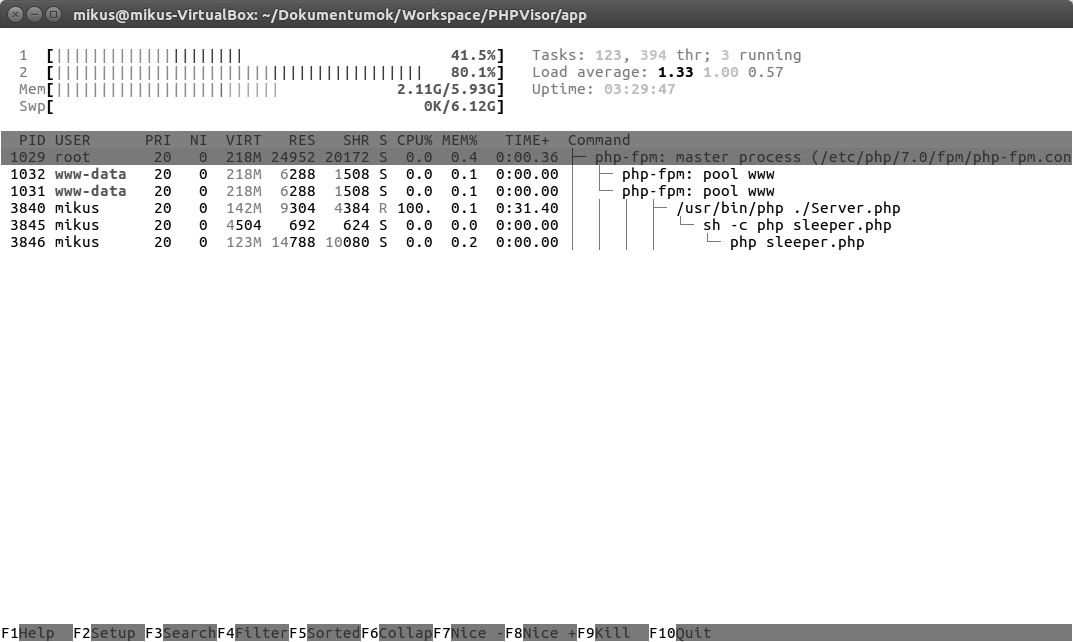
\includegraphics[width=12cm]{pics/htop.png}
	  \caption{Folyamatkezelőben láthatjuk (htop), hogy a program a háttérben tovább fut.}
  \end{figure}
  
  Ilyenkor a program működésének állapotairól csak a naplóbejegyzések segítségével tájékozódhat a felhasználó. 
  \paragraph{}
  Ahhoz, hogy a program működése jobban követhető legyen, a \textit{nodaemon} illetve a \textit{print\_log} opciók megadására/engedélyezésére van szükség. Ekkor jobban megfigyelhető a progam működése közben, ugyanis a nodaemon beállítással, az előtérben, azaz az aktuális terminál ablakon fut az alkalmazás, továbbá a printLog-gal elérhetjük, hogy az  aktuális naplóbejegyzéseket a terminálra is kiírja a program.
Így valós időben megfigyelhető az alkalmazás.
\subparagraph{Megyjegyzés:}
A printLog opció nem használható a háttérben való futtatás esetén, mivel az \textit{echo} függvény arra a terminálra írná az üzeneteket, amelyről leválasztottuk a programot.

  \begin{figure}[ht]
  \centering
  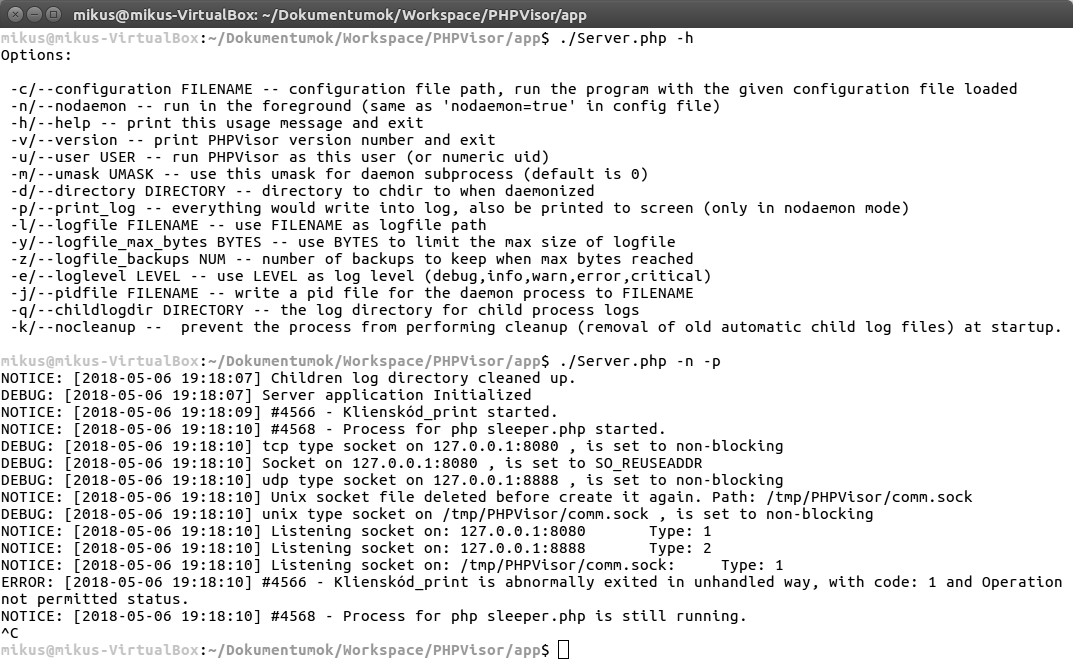
\includegraphics[width=14cm]{pics/run_print.png}
	  \caption{Az alkalmazáson belüli súgó, illetve  a program futásának követésére szolgáló funkciók szemléltetése.\newline}
      \label{fig:run_print}
  \end{figure}

A \ref{fig:run_print}. ábán látható, hogy miután elindult a program, sorban jelennek meg a fontosabb műveletekhez kapcsolódó rendszerüzenetek. A program a beállított naplózási szintnek megfelelő időbélyeggel ellátott bejegyzéseken keresztül leírja mikor inicializálja magát a szerver komponens, milyen folyamatokat indított el a rendszer, milyen portokat nyitott ki, illetve melyeken hallgat. A naplókon nyomon követhetőek \textit{debug} naplózási szinttel, a klienssel való kommunikáció nyomai is. A naplók rögzítik mikor egy kapcsolat létrejön, illetve a kommunikáció tárgyát képező üzeneteket is (\ref{fig:runcon}. ábra).
  \begin{figure}[ht]
  \centering
  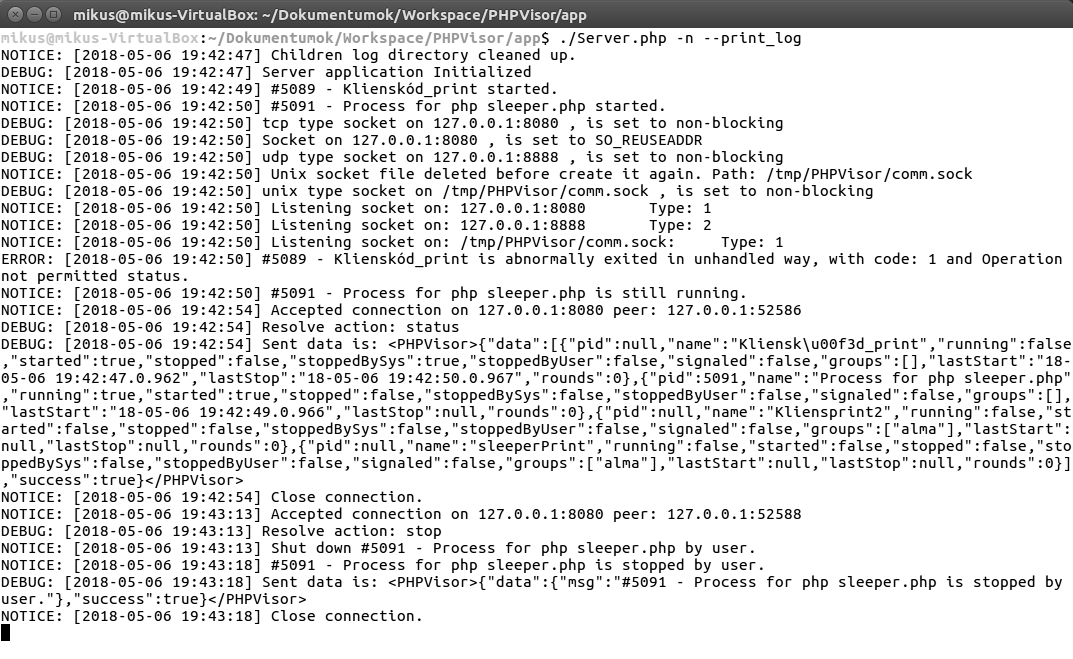
\includegraphics[width=14cm]{pics/runcon.png}
	  \caption{A naplóbejegyzéseken nyomon követhetőek a klienssel kommunikált üzenetek is. \newline}
      \label{fig:runcon}
  \end{figure}

  \subsubsection{Hibaüzenetek}
  \paragraph{}
 Mindkét program (szerver-kliens) kivételek, azaz exception-ök segítségévél jelzi hibaállapotait. A kivételek jellemzően adatbeviteli vagy kommunikációs mechanizmusokból eredhetnek.  A kivétel keletkezése azonnal leállítja a program futását. Amennyiben nem konfigurációs hiba keletkezik, a rendszer az okozó kivételt a napló végére írja, majd leáll.	
 A szerver komponens lehetséges hibaüzenetei:
 \begin{itemize}
 \item \textit{InvalidArgumentException:} Olyan kivételek, amelyek azt hivatottak jelezni a felhasználónak, hogy  konfiguráció során invalid adatot adott meg a megjelölt helyen. 
 \item \textit{RuntimeException:} Ezeket a kivételeket, akkor dobja a program, ha valamely PHP-s függvény nem az elvárt működést produkálja. Ez lehet akár az, hogy az operációs rendszer már nem tud \textit{fork}-olni, de akkor is ilyen típusú hibát kapunk, amennyiben kommunikációs port megadása nélkül indítanánk a programot.
 \end{itemize}
  \begin{figure}[ht]
  \centering
  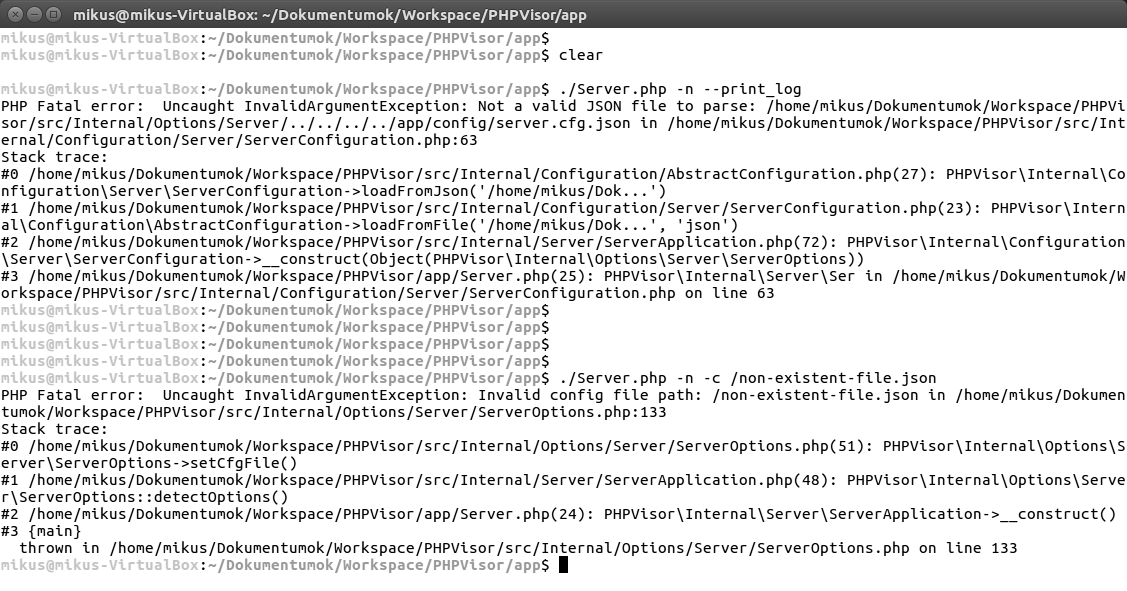
\includegraphics[width=14cm]{pics/runerr.png}
	  \caption{Példa helytelen konfigurációs adat megadásakor keletkező kivételekre. \newline}
      \label{fig:runerr}
  \end{figure}
  
  \pagebreak
\subsection{Client}
\subsubsection{Konfiguráció}
\paragraph{}
A kliens komponensnek lényegesen kevesebb konfigurálási lehetősége van, mint a szervernek. Itt a konfigurációban kvázi az előre egyeztetett adatokat találhatjuk, amelyet a kliens a szervertől kap. A formátuma szintén JSON, illetve a megfelelő szabályok itt is érvényesek. A példa (alapértelmezett) konfigurációs állományt, a már említett \textit{config} könyvtárban találjuk. Definiálásra kerülnek a következő opciók:
\begin{itemize}
\item serverUrl : Ezen beállítás határozza meg azt a kommunikációs címet, amelyre szerenténk csatlakozni. Amennyiben TCP kapcsolatot határozott meg a szerver, úgy elég megadni az IP/port párost a szokásos alakban. (Például: \verb|"127.0.0.1:8080"|). Ha UDP vagy Unix socketen keresztül csatlakozna a kliens, akkor a protokollt is a címbe kell írni. UDP esetén \verb|udp://127.0.0.1:8888|, Unix socketnél \verb|"unix:///tmp/PHPVisor/comm.sock"|. Ez utóbbinál a port szám jellmezően elhagyható, hiszen egy fájlra tett hivatkozásról van szó.
\item username : A felhasználónév alapértelmezett értéke null érték. Viszont csak akkor lesz  a kívánt működésű  a programok kommunikációja, amennyiben az itt megadott érték pontosan megegyezik a szerver konfigurációjában megadottal. A felhasználónév, illetve jelszó párossal minden egyes beérkező kérést authentikál a szerver, így csak a megfelelő információk birtokában nyílik lehetőség a folyamatok tényleges manipulációjára. (Legfeljebb 20 karakter hosszú lehet.)
\item password : A felhasználónévhez hasonlóan, ennek is a szerveren megadott adattal kell egyeznie. (Legfeljebb 20 karakter hosszú lehet.) 
\end{itemize}

\subsubsection{Parancssori konfiguráció}
\paragraph{}
Természetesen a kliens komponens is kihasználja a már említett parancssori opciók nyelvi támogatottságát és a fentebb említett három opció, (plusz a konfigurációs állományt meghatározó opció) szintén megadható a kapcsolók szintjén.
Ekkor a szokásos hierarchia lép életbe a konfigurációs állomány, illetve a konzolos kapcsolók között. (A kapcsolók előnyt élveznek.)
A kliens az alábbi kapcsolókat ismeri: \\ \\
 \begin{tabular}{ c | c | c | l }
 \label{tab:cli}
 \centering
  \textbf{Rövid név} & \textbf{Hosszú név} & \textbf{Paraméter} & \textbf{Funkció} \\ \hline
  c & configuration & FILENAME & A megadott FILENAME \\
  &&& konfigurációs állomány használata. \\ \hline
  h & help & & Kiírja a programhoz tartozó súgó üzenetet, \\
  &&& a parancssori kapcsolókról, leírásukkal. \\ \hline
  l & url & URL & A megadott URL használata \\
  &&& mint serverUrl. A cím, \\
  &&& amelyre a kliens csatlakozik. \\ \hline
  u & user & USERNAME & A jogosultság ellenőrzéshez \\
  &&& használt felhasználónév. \\ \hline
  p & pwd & PASSWORD & A jogosultság ellenőrzéséhez \\
  &&& használt jelszó.\\ \hline
  \end{tabular}
\\
  \paragraph{Paraméterek}
  \begin{itemize}
  \item FILENAME : A szerver konfigurációjának leírásával analóg módon, itt is a kívánt fájl elérési útvonalát határozhatjuk meg. Az alapértelmezett fájl a \textit{config} mappa alatt található \textit{client.cfg.json}.
  \item URL : A konfigurációs részben taglatak szerinti szabályok alapján formázott kommunikációs cím, amelyen keresztül a szerverhez kapcsolódik a kliens.
  \item USERNAME : A megadott felhasználónév, amellyel a kommunikációt szeretnénk végezni. (Legfeljebb 20 karakter hosszú lehet.)
  \item PASSWORD : Az előbbi felhasználónévhez tartozó jelszó. (Legfeljebb 20 karakter hosszú lehet.)
  \end{itemize}
  \subsubsection{Futtatás}
  Az alkalmazás indításához szükséges állomány a \textit{főkönyvtár/app} alkönyvtárában található. Az indításhoz a  Client.php szkriptet kell futtatni, amire két lehetőség adott: A \textit{/app} könyvtárban állva,
  \begin{itemize}
  \item a parancssorba kiadni a \verb|php Client.php| parancsot vagy
  \item a parancssorba kiadni a \verb|./Client.php| parancsot, (amennyiben a \textit{/usr/bin/php} útvonalról elérhető a php)
  \end{itemize}
  A program használati célja, hogy a szerver-komponensen keresztüli kommunikáció során információt szolgáltasson a felhasználójának a szerveren beállított folyamatokról, illetve adott parancsokat közvetítsen feléjük. Az implementált akciólistából válogathat a menün keresztül a felhasználó, amelyet a billentyűzet segítségével irányíthat. Egy lehetőség kiválasztásához a kiválasztott menüpont betű vagy szókódját kell begépelni, majd Enter-t nyomni. Amennyiben ismeretlen opciót választunk a program erről tájékoztatást ad majd újra lehet próbálkozni. Vannak olyan akciók is amelyek további paraméterek megadását követelik (például folyamat indítása név alapján). Ekkor a megfelelő menüpont kiválasztása után a program tájékoztatást ad, arról, hogy milyen értéket vár. A kívánt értéket a billentyűzeten beírva, majd Enter-t ütve lehet az akciónak átadni.
  
    \begin{figure}[ht]
  \centering
  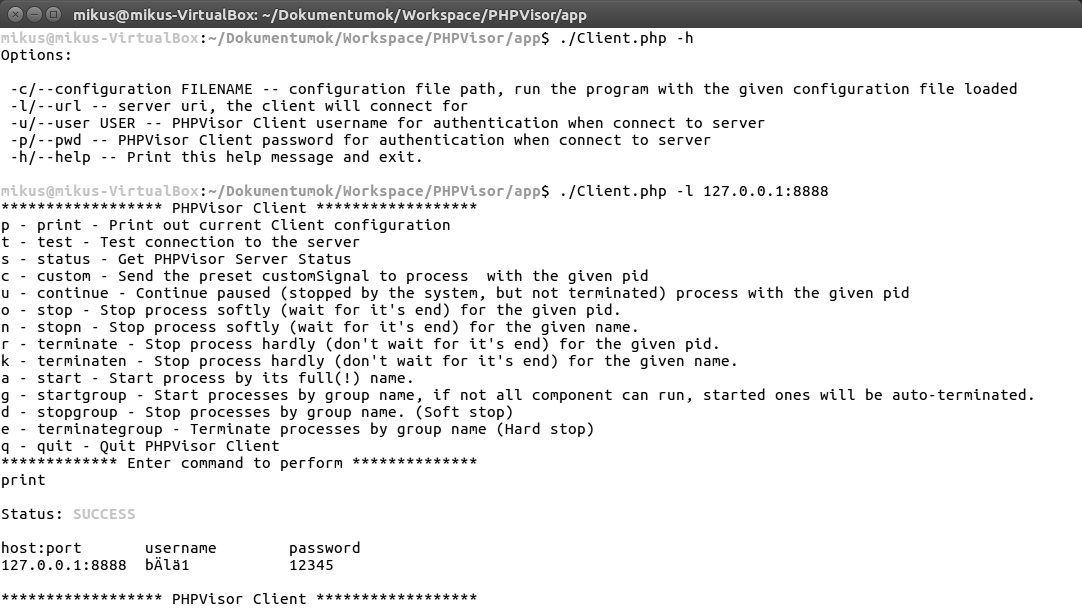
\includegraphics[width=14cm]{pics/cli_h_conf.png}
	  \caption{A kliens program indításának szemléltetése  kapcsolók használatával. A menün keresztül látható milyen utasításokat lehet használni. \newline}
      \label{fig:cliconf}
  \end{figure}
  
  \subsubsection{Működés}\label{sec:cli_funcs}
  \paragraph{}
  A program elindulását követően rögtön kiírja a képernyőre a menü-t, amelynek segítségével tájékozódhat a felhasználó a lehetséges opciókat illetően. Amennyiben a szerver alkalmazás nem fut, úgy a kapcsolódási kísérleteket tartalmazó akciók egy kivétel dobásával közlik, hogy a kapcsolódás meghiúsult. A program lehetőséget nyújt a kapcsolat tesztelésére anélkül, hogy valamely folyamatot érintő akcióval kellene ezt letesztelni.
A program menüpontjai a következők:
\begin{itemize}
\item print : Ezen menüponton keresztül, az aktuális konfigurációt lehet megtekinteni. A program kiírja a csatlakozási pont hivatkozását, a fehasználónevet és a jelszót is a képernyőre. (\ref{fig:cliconf}. ábra)
\item test : Lehetőség van tesztelni a szerverhez való csatlakozás sikerességét. Ilyenkor siker esetén egy üres üzenetet kapunk vissza a szervertől, hiba esetén egy hibajelzést.
\item status : Ezzel az opcióval lekérdezhetőek a szeveroldalon futtatott folyamatok státuszai. A program oszlopokba szedve kiírja a képernyőre a futtatott folyamatok azonosítóit, illetve állapotukat is. (Az egyes oszlopok részletes jelentésének leírása a \ref{par:mean}. pont alatt olvasható.)
\item custom : A funkció egy előre (szerver oldalon, a folyamat konfigurációjában) meghatározott szignált küld az adott folyamatnak.
\item continue : Amennyiben az operációs rendszer egy folyamatot megállít (szünetelteti), ezzel a funkcióval egy folytatásra késztető szignált küld az adott folyamatnak.
\item stop : A kliensben a stop fogalma eltér a megszokottól. Itt nem áll meg a folyamat tényleges futása, hanem a \verb|proc_open| függvény hívásával a program egy futásának a végét megvárva leállítódik. Ezen opció lehetőséget nyújt egy ilyen típusú leállításra a folyamat pid-a alapján.
\item stopn : Az előbb leírt működést produkálja, csak az előzővel ellentéteben itt a program neve alapján van lehetőség leállítani a folyamatot, nem a pid-a alapján.
\item terminate : Ezen funkció a stop működésnek a kényszerített verziója. A megadott pid-ú folyamat terminálására van lehetőségünk a \verb|proc_terminate| függvény segítségével, amely a folyamat konfigurációjában megadott termináló szignált küldi a folyamatnak, ezzel az azonnali megállítását okozva.
\item terminaten : Az előbb említett terminálási funkció azzal a kivétellel, hogy itt a folyamat neve alapján van lehetőségünk terminálni.
\item start : Ez az opció lehetőséget ad számunkra, hogy a szerveroldalon előre megadott folyamatok közül elindítsunk egyet. Az akciónak megadott folyamatnév alapján kerül a folyamat elindítása. (A teljes név megadása szükséges, ezért célszerű lehet nem a rendszerre bízni, a process nevek automatikus kiosztását.)
\item startgroup : A program a szerver leírásban említett címkék/csoportnevek alapján is el tud indítani, esetleg megállítani programokat.  A program a megadott csoportnév alapján a konfiguráció sorrendjében elindítja a folyamatokat. Amennyiben egy folyamat már futott a csoportból, ahhoz nem nyúl. Amennyiben az adott kérés során indított folyamatok közül valamelyiket nem sikerült elindítani, a szerver leállítja ezeket az elindított folyamatokat is. (Amelyek a kérés előtt is futottak, azokat nem.)
\item stopgroup : Ezen lehetőség segítségével a fentebb említett csoportnév alapján lehet kérni azok (soft) normál leállítását. (Hasonlóan a stop lehetőséghez, csak itt csoportnévvel szűrünk a leállítandó folyamatokra.)
\item terminategroup : Ennek a parancsnak a segítségével lehetőség nyílik megadott csoportnév alapján, kikényszerített leállítást kezdeményezni a csoport folyamataira.
\item quit : Ezen menüpont választásával a program kilép. 
\end{itemize}
 \begin{figure}[ht]
  \centering
  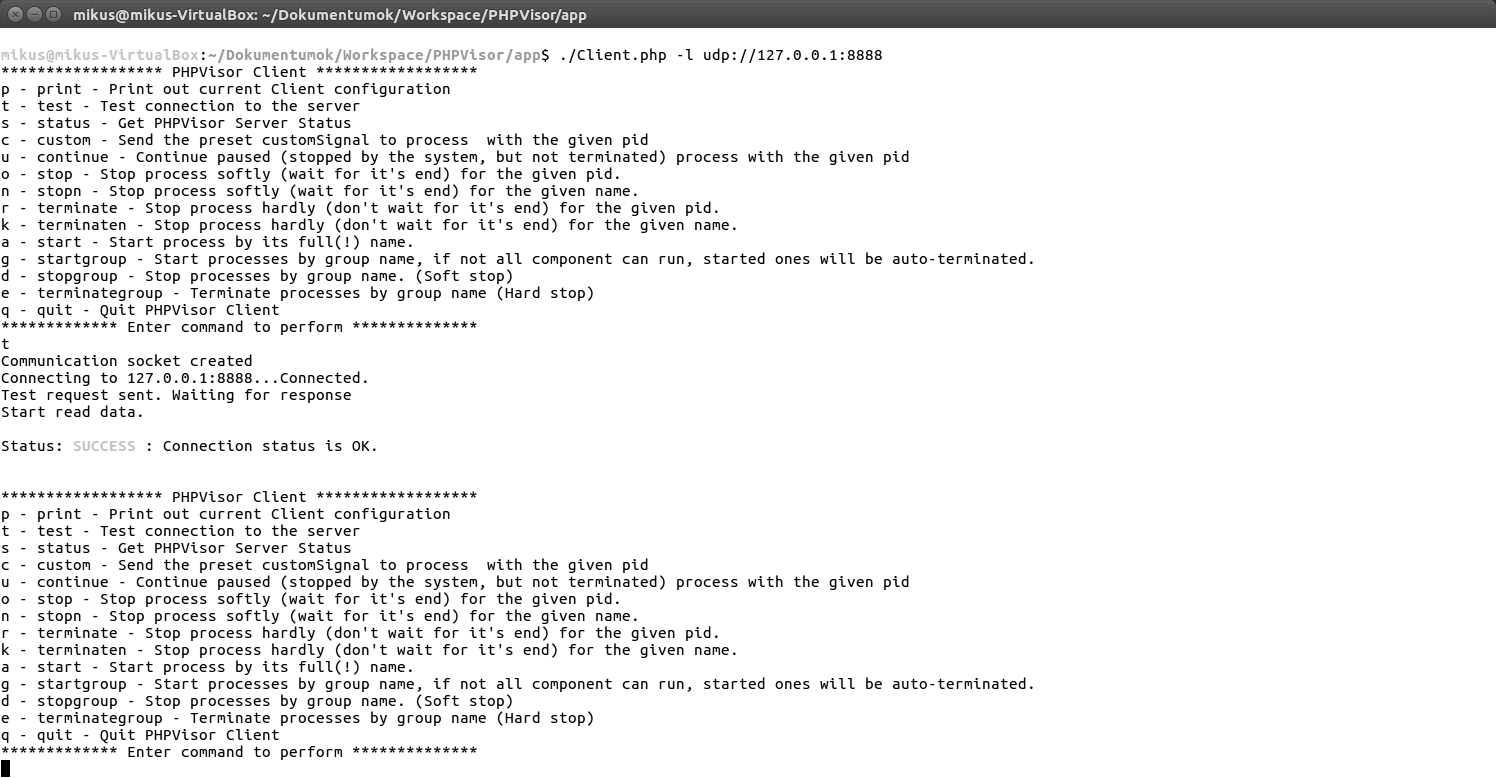
\includegraphics[width=15cm]{pics/test.png}
	  \caption{A kliensnek, a szerverrel való kapcsolatának tesztelése a kliens program \textit
      {test} opciója alapján.}
      \label{fig:clitest}
  \end{figure}
  
  \pagebreak

\subsubsection{Felület értelmezése}\label{par:mean}
 \begin{figure}[ht]
  \centering
  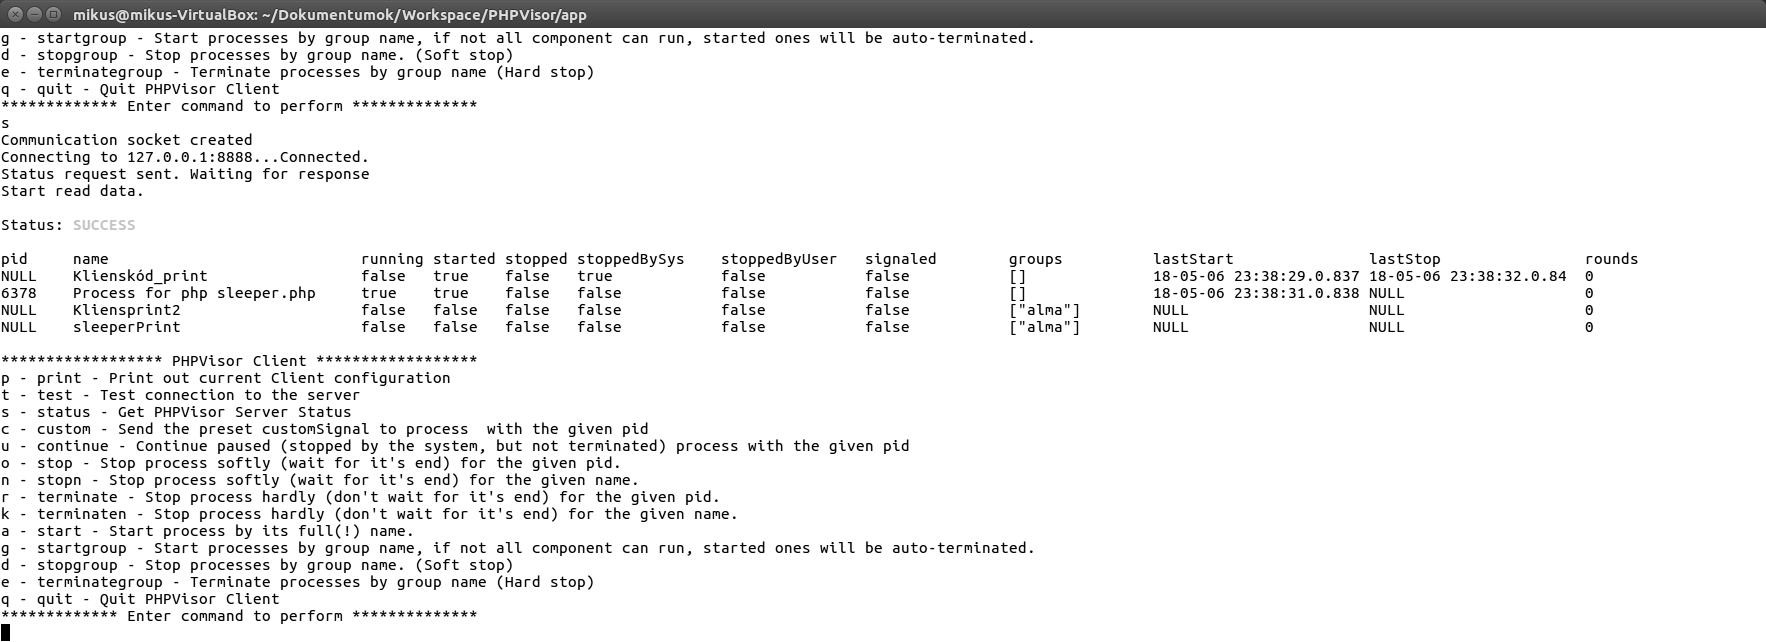
\includegraphics[width=15cm]{pics/stat.png}
	  \caption{A kliensen keresztül lekérhető az aktuálisan konfigurált folyamatok állapota.}
      \label{fig:clistat}
  \end{figure}
  
  A \ref{fig:clistat}. ábrán látható, amikor a kliens lekérdezi az aktuális folyamatok állapotát. Ekkor összesen 12 oszlopban tájékoztatást kapunk a legfontosabb információkról, állapotokról. Az első oszlopban látható a folyamatok \textit{pid}-a, ha van. Amennyiben egy folyamat éppen nem rendelkezik pid-val, úgy NULL-ként jelenik meg, ez jelzi, hogy a folyamat nem fut. Mivel nagyon gyorsan lefutó folyamatok is lehetnek a konfiguráció részei, ezért ez az adat nem tekinthető aktuálisnak. Ez az oka amiért nem csak az azonosító szerinti manipulációt, de a név szerintit is támogatja a rendszer.
  A második oszlopban a program megnevezése található (\textit{name}). A formázott kiíratásnak karakterszám-béli korlátja is van, ezért ajánlott rövid és tömör elnevezéseket használni a folyamatokhoz. (Érdemes azért is ügyelni a rövid, egyértelmű és lehetőleg egyedi nevek használatára, mivel a programban nincs implementálva egyediséget ellenőrző logika, ezért a név alapján talált első azonosított folyamattal fog a rendszer dolgozni, ha az kérdéses helyzetbe kerülne.)
  A harmadiktól a nyolcadik sorig a következő állapotjelző információkat találhatjuk:
  \begin{itemize}
  \item running : Arról ad tájékoztatást, hogy a megadott folyamat fut-e vagy sem. 
  \item started : Ha igaz, akkor az alkalmazás el lett indítva, de nem feltétlenül fut. Ekkor érdemes tüzetesebb vizsgálatnak alá vetni a folyamat saját naplóját. (A természetes megállás újraindításkor megfelelően kapcsolja ennek az értékét.)
  \item stopped : Amennyiben az operációs rendszer megállítja a folyamat futását, T jelzésű (stopped) állapotba helyezi a folyamatot, ekkor a folyamat tulajdonképpen tovább fut. Ilyenkor lehetőség van megkísérleni a folyamat folytatását a megfelelő folytatást jelentő szignál küldésének segítségével, amire a program lehetőséget is ad.  
  \item stoppedBySys : Amennyiben igaz, az a következőket jelentheti. Ha a program normálisan (a tőle elvárt módon) állt meg, ez az érték igaz lesz miközben a running, és a started hamisra vált, továbbá a rounds oszlopba eggyel nagyobb szám kerül. Ha program abnormálissan állt meg, (például egy szignál kényszerítette megállásra) az értéke igaz lesz, ahogyan a signaled oszlop értéke is.
  \item stoppedByUser : Ez az állapotjelző azt fejezi ki, hogy a felhasználó a kliensen keresztül állította le a programot. (Vagy terminálta azt.)
  \item signaled : Amennyiben igaz, a programot valamely szignál megállásra késztette. (Ez az érték újra hamisra vált, ha egy stopped folyamatnak folytatási kérelmet küldünk.)
  \end{itemize}
  \paragraph{}
  A képernyőre írt információk között, a \textit{groups} kulcs alatt megjelenik az egyes folyamatok címkelistája is, amely segítséget nyújthat, amennyiben csoportnév alapú műveleteket szeretnénk végrehajtani. 
  További két oszlopban időbélyegekkel ellátott jelzőket találhatunk, a \textit{lastStop} értéke bárminemű fentebb említett leállás legutóbbi idejét, míg a \textit{lastStart} a legutóbbi indításának időpontját szimbolizálja.
  Az utolsó oszlopban a már említett \textit{rounds}, az egyes futásokat számlálja. Egy teljesértékű, normális lefutás e számláló eggyel való növekedését okozza.
 \\
 A státuszinformációk kinyerésén kívül folyamatok futását befolyásoló parancsok közlésére is van lehetőség. Ezek paraméterhez kötött akciók, amelyek esetében a paraméterek, az akció hatáskörébe eső folyamatokat határozzák meg.
 \paragraph{}
 A szerverrel való kommunikáció eredményéről a kliens minden esetben tájékoztat. \textit{Success} állapottal jelzi, amennyiben a kérés sikeresen célt ért, végrehajtódott és a megfelelő sikeres válaszüzenetet kapta vissza.(\ref{fig:succ}. ábra) 
Amennyiben valamely olyan eset lépett fel amelyet a szerver hibásnak ítélt meg, (például elrontott felhasználó-jelszó páros), a válaszban érkező hibaüzenetet a kliens az \textit{Error} állapottal jeleníti meg (\ref{fig:err}. ábra).
  
  \subsubsection{Hibaüzenetek}
  \paragraph{}
 Abban esetben, ha üzenetváltás során elszállna/leállna a szerverkomponens, miközben a kliens a válaszra vár, az nem kapja meg a megfelelő méretű üzenetet, s \textit{Error} státuszú hibaüzenet ír ki a képernyőre, miszerint nem tudta megfelelően átvenni az üzenetet a szervertől. A kliens 60 másodpercig vár egy-egy kérés után a válaszra, és amennyiben az lejár, s nem érkezik megfelelő válasz, ugyanúgy az előbb említett hibaüzenet jelenik meg a képernyőn. 
 
  A program működése során nem csak az imént említett hibák jelenhetnek meg. Az alkalmazás a szerver komponenshez hasonlóan kivételekkel jelzi, amennyiben a kiépített kommunikációs csatáronán hiba lépett fel. 
  A \textit{Connection refused} kódú hibaüzenet (\ref{fig:connref}. ábra), azt jelenti, hogy a kliens nem tud kapcsolatot létesíteni a kívánt host-tal (például amennyiben a szerver nem fut és csatlakozni próbálunk rá), míg a \textit{Not connected} kódú hibaüzenet (\ref{fig:notconn}. ábra) azt hivatott jelezni, hogy a kliens és a szerver között megszakadt a kommunikációs kapcsolat.
  
 \begin{figure}[ht]
  \centering
  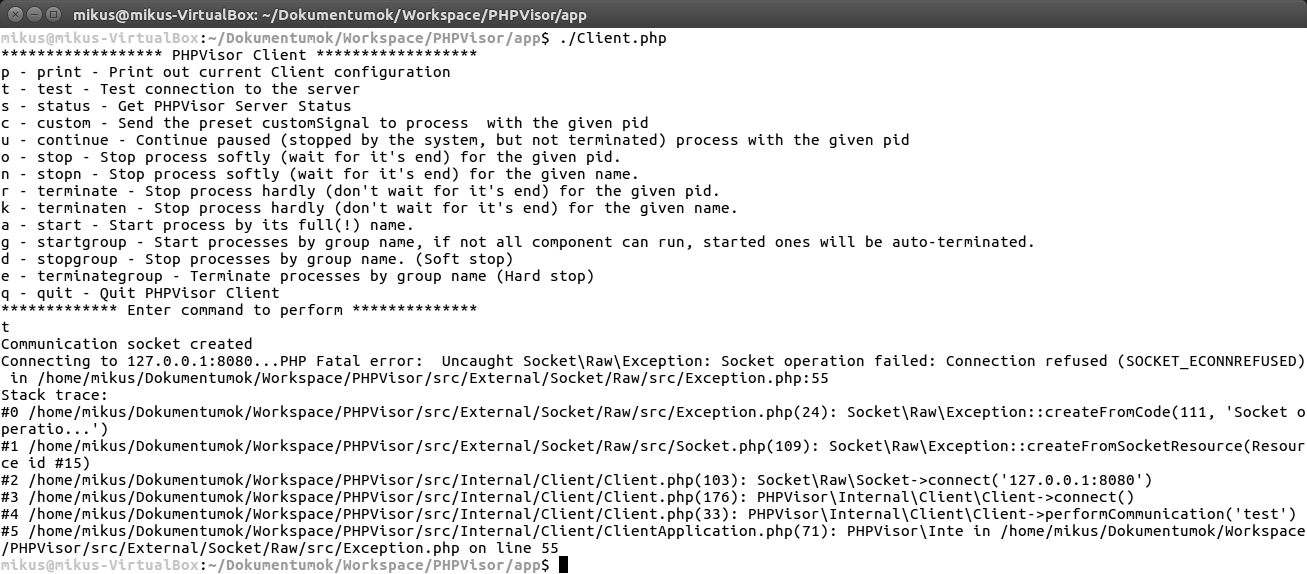
\includegraphics[width=15cm]{pics/connref.png}
	  \caption{Példa a \textit{Connection refused} kivétel megjelenésére.}
      \label{fig:connref}
  \end{figure}

   \begin{figure}[ht]
  \centering
    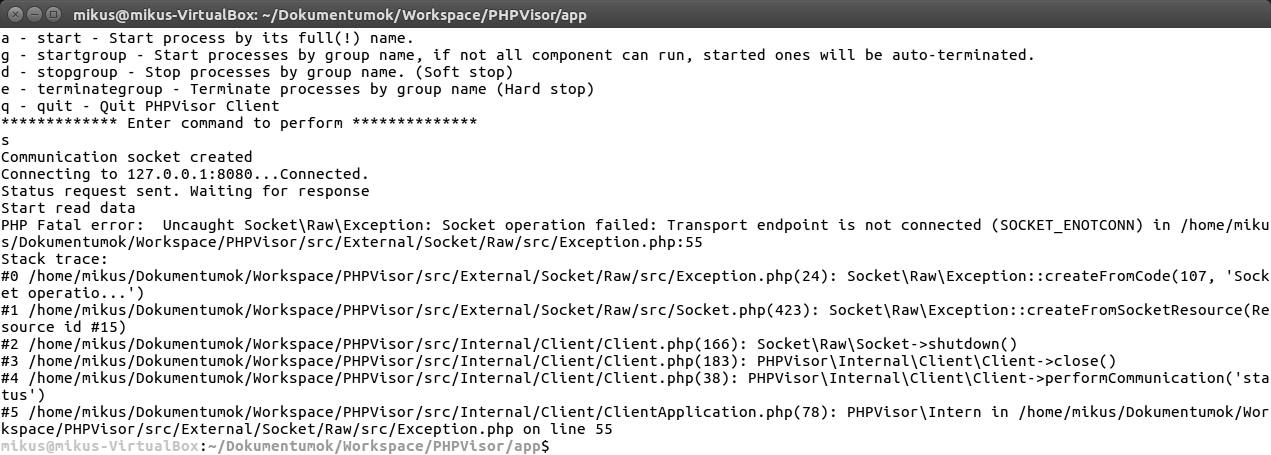
\includegraphics[width=15cm]{pics/notconn.png}
	  \caption{Példa a \textit{Not connceted} kivétel előfordulására.}
      \label{fig:notconn}
  \end{figure}
  
     \begin{figure}[ht]
  \centering
    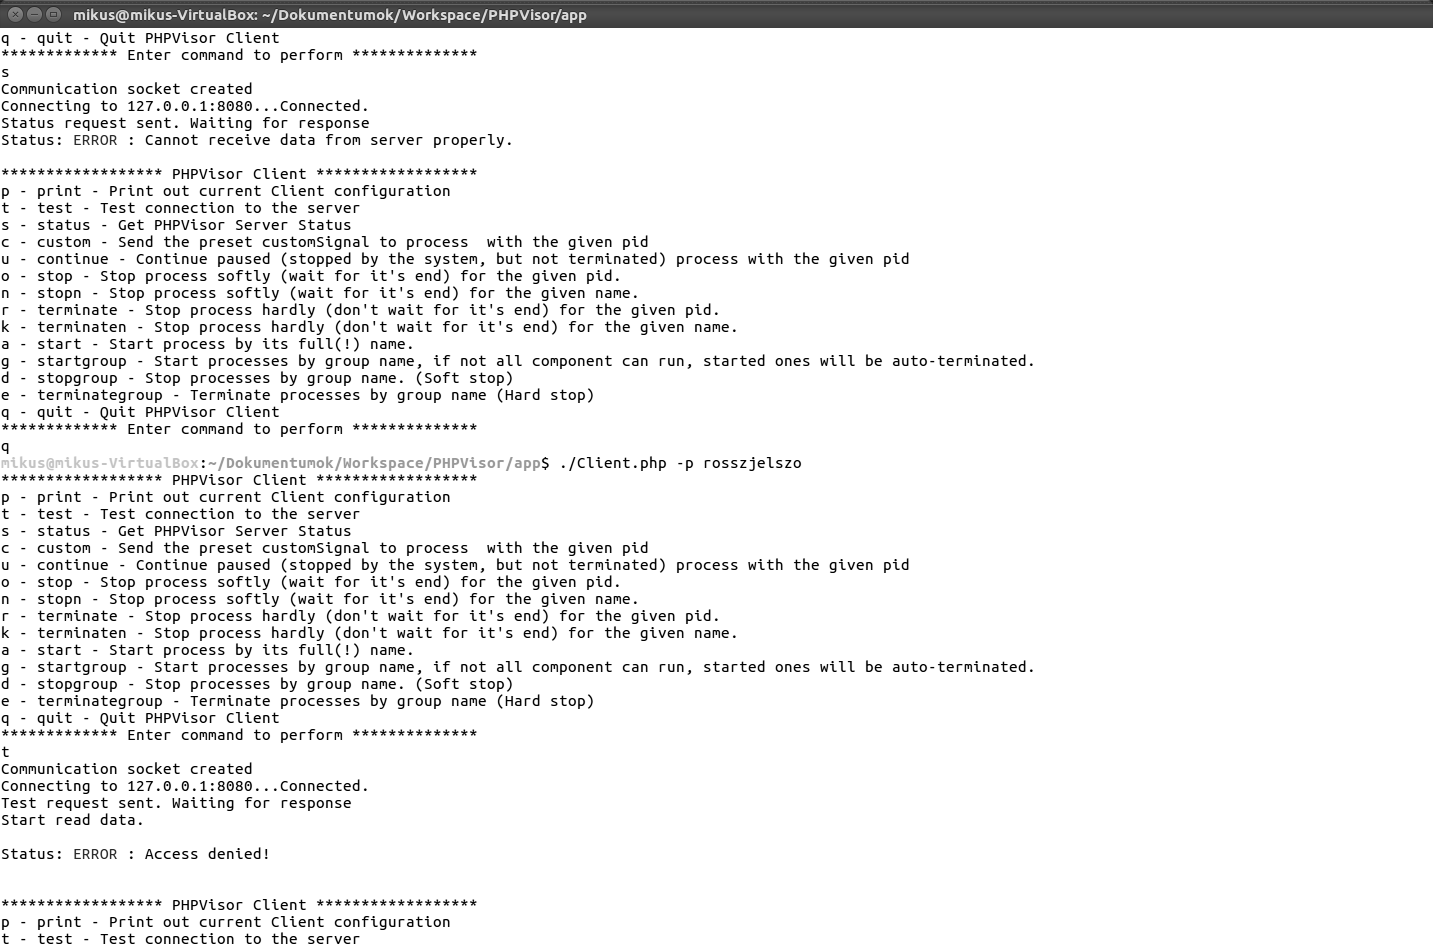
\includegraphics[width=15cm]{pics/err.png}
	  \caption{Példa hibás üzenet fogadásakor vagy timoutkor keletkező hibára, illetve téves jogosultsági adatok esetén keletkezp hibára. }
      \label{fig:err}
  \end{figure}
  
     \begin{figure}[ht]
  \centering
    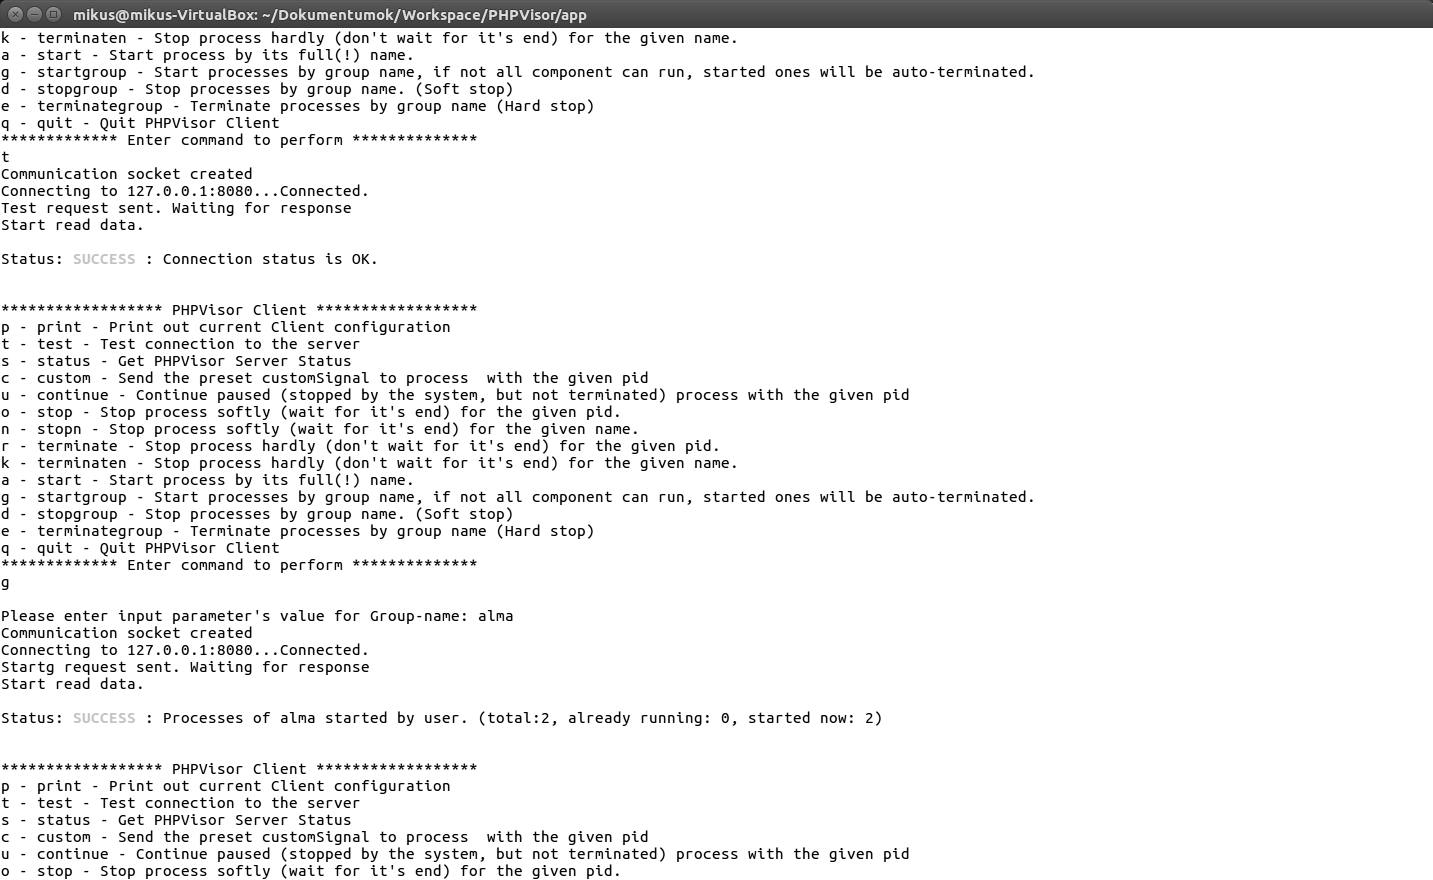
\includegraphics[width=15cm]{pics/succ.png}
	  \caption{Példa sikeres üzenetváltásokra.}
      \label{fig:succ}
  \end{figure}
  \pagebreak
\chapter{Fejlesztői dokumentáció}
\paragraph{}
Ezen fejezetben bemutatásra kerül a programok szerkezete, felépítése, illetve a megvalósításnak bizonyos elemei is. Továbbá megemlítésre kerülnek komolyabb problémák, amelyek a rendszer körül adódhatnak, érdekesebb algoritmusok, nyelvi korlátok és az is, hogy az alkalmazások milyen objektumokból épülnek fel. Megjegyzés szintjén jövőbe mutató javaslatokat, ötleteket is közlök, amelyek útmutatásul szolgálhatnak a későbbi fejlesztési időszakokban.
\paragraph{}
Az alkalmazások tervezése és megvalósítása objektum-orientált szemléletben történt, aminek eredményeképp sokféle osztály került megvalósításra. Ezek hierarchiába, illetve öröklődési láncokba szervezve működnek együtt.
\paragraph{}
A fejlesztés során a kommunikációs alapokhoz egy alacsonyszintű külső könyvtárat használtam, amely egy minimális OOP szemléletű réteget helyez a PHP szolgáltatta socket függvények fölé. A könyvtár nyílt forráskódú, MIT licensszel ellátott project, amely megtalálható a GitHub-on.\textsuperscript{\cite{cluesocket}} Segítségével könnyedén megvalósíthatóak a szerver, illetve a kliens objektumok, amelyek a kommunikáció alapját képezik. Használatát tekintve egyszerű. Egy ún. Factory objektumon keresztül példányosítja a megfelelő komponenst, ami a Socket osztály egy példánya.
A külső forrásanyag, teljes project-ként megtalálható az alkalmazás \textit{src} mappájának \textit{External} almappája alatt.
\pagebreak
\section{Tervezés}
\paragraph{}
A  feladat részletes leírása a \ref{par:feladat}. pontban található. A program architektúrája miatt két alapvető egységre bomlik: kliensre és szerverre. A szerver egy olyan program, amely futása közben felhasználói interakciót nem biztosít, így tulajdonképpen csak egy konfigurálási réteggel lép kapcsolatba a felhasználó. A kliens ezzel szemben, egy főképp felhasználói interakcióra épülő alkalmazás, amelynek lehetőséget kell biztosítania az elvárt akciók végrehajtására és közlésére a szerver felé.

Mindkét program egy-egy objektumént való reprezentálásával, egy könnyen alkalmazható ún. alkalmazási réteg jön létre. Ez azt jelenti, hogy az egyes futást kiváltó állományokban, csupán a megfelelő alkalmazás-objektum példányosítására majd elindítására van szükség.
Ezen alkalmazásrétegbe épül be a konfigurációs-réteg és a program lényegét adó metódusok is. 
Az alapkoncepciója a programoknak, hogy az \textit{Application} programváz a megfelelő \textit{AbstractOptions} tulajdonságokkal ruházza fel magát a beállítások meghatározását követően.
     \begin{figure}[ht]
  \centering
    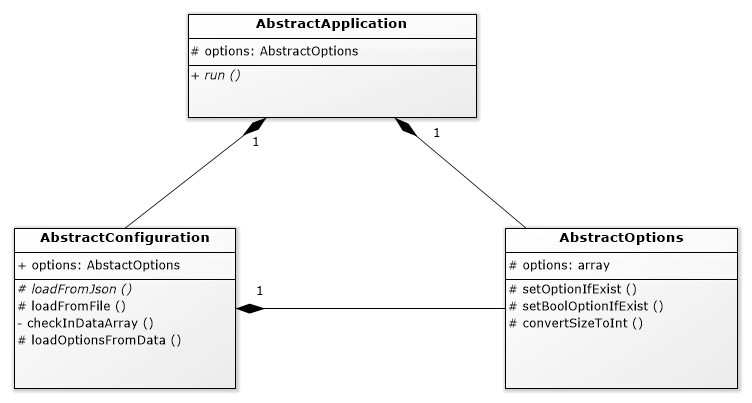
\includegraphics[width=15cm]{pics/abstracts.png}
	  \caption{A programok alapstruktúrájának vázlata.}
      \label{fig:abstract}
  \end{figure}
Az \textit{AbstractOptions} reprezentálja az alkamazások által használt beállításokat, amelyket az \textit{Application} detektál induláskor. Ezután a megfelelő alkalmazásobjektum létrehozza a lényeget képező objektumot (Kliens objektum - Szerver objektum). Ezen objektumok, a hozzájuk tartozó \textit{AbstractConfiguration} segítségével jönnek létre, ugyanis ezen konfigurációs réteg valósítja majd meg a fájlból történő információ kinyerését, amely adatokkal aktualizálja a megfelelő \textit{AbstractOptions} objektumot.
A konfigurációs, illetve opciós szintek elkülönítésére azért van szükség, mert a program indításakor megadott esetleges opciók között lehetnek olyanok is, amik függetlenek az elvárt szerver- vagy kliensműködéstől (például a \textit{help} menü megjelentése, majd kilépés funkció). Továbbá az egymást átfedő beállítások kezelésére is megoldást nyújt a struktúra, mert ezáltal elkülönítve töltjük fel információval az opcióhalmazt például a konzolról, illetve fájlból.
A \ref{fig:abstract}. ábrán megjelenő gráf, alsó útja - az options-től a configuration-ig, majd tovább az application-be - a fájlból való konfiguráció, a jobb oldali útja - az options-ből egyenesen az application-be - a parancssori konfiguráció egy interpretációja.
     \begin{figure}[ht]
    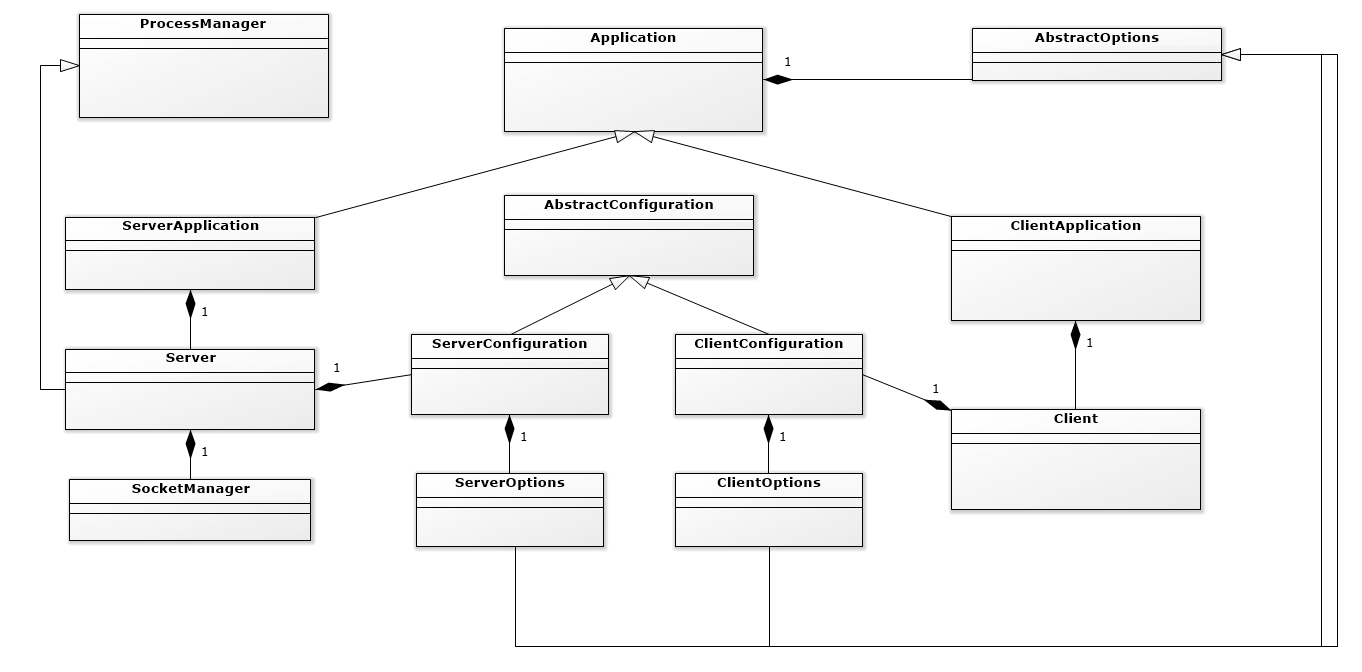
\includegraphics[width=16cm]{pics/classes.png}
	  \caption{A rendszerben előforduló fontosabb objektumok hierachiáját és kapcsolatát szemléltető ábra.}
  \end{figure}
\subsection{Server}
  \paragraph{}
  A szerver három legnagyobb feladata a socketek kezelése, a folyamatok felügyelete és a beérkező kapcsolatok lebonyolítása. A socketet létrehozása a SocketManager objektum feladata, amelyet a Server objektum konstruálásakor hozunk létre. A Server önmagában a ProcessManager osztályból származik, aminek feladata a folyamathoz kötődő funkciók kezelése, mint például folyamatok elindítása, megállítása. A klienssel való kommunikációt önmagában valósítja meg a Server.
  
  \subparagraph{Megjegyzés:}Javaslat fejlesztéshez, hogy az imént említett kommunikációs műveletek leválasztásra kerüljenek a Server objektum törzséről.
  \paragraph{}
Ezen felül rendelkeznie kell a feladatban definiált naplózási funkciókkal, amelyeket a \textit{Logger} objektum hivatott kezelni. A Logger feladata a megfelelő naplózási opciók (\textit{LogOptions}) szerinti naplóbejegyzések készítése. (Ezen bejegyzéseket szintén  a szerver vezérli).

\paragraph{}
  A szerver komponens önmagában használható funkciókat nem biztosít, csak a kliens általi vezérlés lehetséges. A kliensoldalról érkezett üzeneteket JSON-ben kódolva kerülnek a szerveroldalra, ahol a megfelelő feldolgozó műveletek és a válasz előállítása után szintén JSON-ben a szerver válaszol a kliens-nek.
  
\subsubsection{Felhasználói esetek}
A felhasználói eset diagrammok segítségével postosabb képet kaphatunk a komponens műkődésével kapcsolatban.

  \begin{figure}[ht]
       \centering
    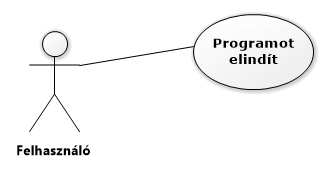
\includegraphics[width=6cm]{pics/uc.png}
	  \caption{Ömagában a szever nem rendelkezik különösebb interakciót igénylő használati esetekkel, a program elindításán kívül.}
  \end{figure}
  
    \begin{figure}[ht]
       \centering
    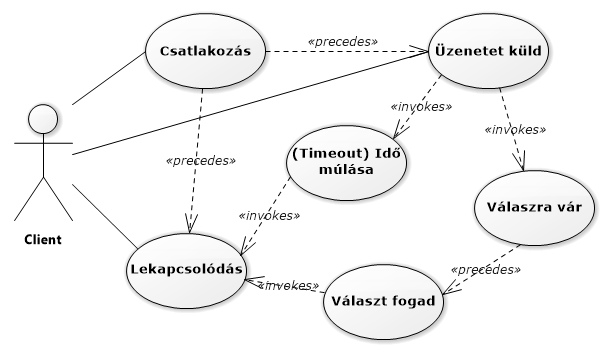
\includegraphics[width=15cm]{pics/client_serv_u_c.png}
	  \caption{Amennyiben a kliens-t tekintjük actornak, úgy több használati eset is szemléltethető.}
  \end{figure}
  
\subsubsection{Osztályok}
A szerver az alábbi osztályokból épül fel:
  \paragraph{ServerApplication}
  
  Ezen osztály képezi a szerver komponens alkalmazás rétegét. Az objektum feladata érzékelni a parancssori beállításokat. Ha a verziót kérik le, akkor az ApplicationVersion osztályból kinyerhető az aktuális verziószám, ha a súgót, a paraméterekhez írt segédleírás íródik aki a képernyőre. Mindkét esetben a program leáll bármilyen folyamat indítása nélkül.
  Egyéb esetben a program létrehoz a kinyert opciókból egy ServerConfiguration-t, amelyet aztán a Server létrehozásához használ fel.
  \paragraph{ServerOptions}
  Ezen osztály tartalmazza a lehetséges Server beállításait. Az osztály felel a parancssori kapcsolók kinyeréséért is. A legtöbb argumentum rendelkezik alapértelmezett értékkel, ami felülírásra kerül amennyiben egy adott opciót megadunk.
  \paragraph{ServerConfiguration}
A beállításokat közvetítő osztály, az \textit{AbstractConfiguration} leszármazottjaként egy \textit{AbstractOptions} paraméterből konstruált osztály, ami felhasználva az aktuális opciókat (konfigurációs fájl) betölti a fájlban található beállításokat. A ServerOptions, LogOptions, ProcessOptions osztályokat látja el adattal.
  \subparagraph{Megjegyzés:}
  Az alkalmazás jelenlegi funkcionalitásához képest a jövőben, akár célszerű lehet más formátumú konfigurációs fájlok feldolgozását is támogatni. Ekkor az osztályban egy újabb metódus felvitelére van csak szükség, a \verb|loadFromJson| metódus mintájára.
  \paragraph{Server}
  A komponens magját képező objektum. Ezen objektum kezeli a fontosabb rendszernaplókat, és írja azokat a Logger segítségével. Az osztály legfontosabb metódusai a futást jelző \verb|run| és a \verb|runForever|. A run elindítja a szerver által várt működéssorozatot:  elindulnak a megfelelő folyamatok és kinyílnak a kommunikációs ablakok. A runForever metódus feladata pedig, hogy egy végtelen ciklus segítségével minden interakcióban megvizsgálja a socketeket és a programokat. Továbbá az osztályban definiáltak a beérkező üzeneteket feldolgozó metódusok, ahogyan a kommunikációs interfészt kiszolgáló funkciók is.
  Ezen kívül a szerver demonizálható is, így az ezt megvalósító függvény is itt van.
  
    \begin{figure}[ht]
       \centering
         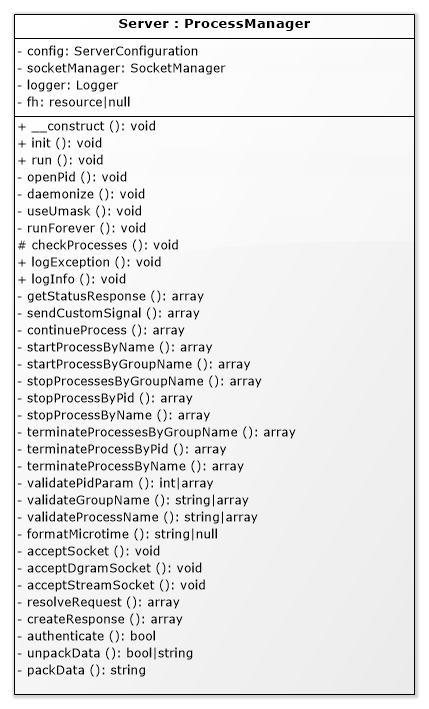
\includegraphics[width=8cm]{pics/serv.png}
	  \caption{A Server osztályt ábrázoló diagramm.}
  \end{figure}
  
  \paragraph{ProcessManager}
  Az előbb taglalt Server objektum őse. Az objektum rendelkezik két tárolóval. A \textit{pool} nevű gyűjtőbe, minden megkreált Process objektum bekerül. A \textit{runningPool}, pedig az aktuálisan futó folyamatok tárhelye. Ez a réteg biztosítja a Server számára, a megfelelő akciók működését. (elindítás, leállítás, terminálás)
  \paragraph{ProcessOptions}
  Ez az osztály reprezentálja, a megadható folyamat-beállításokat. Ezen opció-réteg-beli objektumok feladata, az adott lehetőségek beállítása, illetve validálása.
  \paragraph{Process}
  Az egyes futttandó folyamatokat reprezentálja ez az osztály. Feladata alapvető kezelési funkciók biztosítása (elindíáts, leállítás), továbbá a folyamatok állapotainak változását aktualizáló működés megvalósítása.
  
  \begin{figure}[ht]
       \centering
         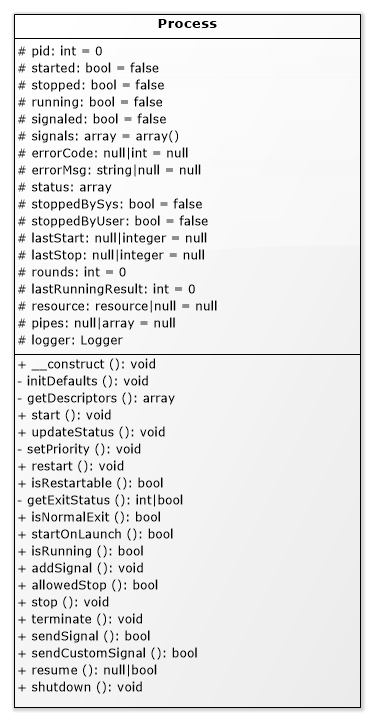
\includegraphics[width=8cm]{pics/proc.png}
	  \caption{A Process osztály fontosabb metódusait ábrázoló diagramm.}
  \end{figure}
  
  \paragraph{ApplicationVersion}
  A szerver alkalmazás verziószámát szolgáltató objektum. A feladata a verziószám meghatározása. Jelenleg a működése abból áll, hogy a megfelelő verzófájlból kiolvassa az verziót képző string értéket.
  \subparagraph{Megjegyzés:} Fejlesztési lehetőségként feltüntetném, hogy az osztály könnyen tovább bővíthető lehetne, valamely olyan szogáltatással, amivel a megfelelő verzióérték automatikusan lekövetését garanatálja. Ezzel tulajdonképpen a verzió, verziófájlba történő írásást automatizálnánk.
  \paragraph{SockerManager}
  A socketek létrehozásáért felelős manager osztály, ami a socket objektumokkal kapcsolatos kollektív műveleteket implementálja, mint például a konfiguráció alapján való létrehozás, beállítás vagy hallgatás (STREAM\_SOCKET esetén). Az objektum naplózási funkcióit a Server objektumtól átvett Logger osztály segítségével valósítja meg. Az objektum a socketek felépítésekor a megadott beállításokon kívül a nem blokkoló tulajdonság beállítását is eszközöli. Erre azért van szükség, hogy a szerver alapműködését garantáló főciklus futása ne blokkoljon amikor a socketen kommunikáció zajlik.
  Az osztály a külső (\textit{External}) könyvtár \textit{Factory}-ából származik le. Ennek oka, hogy a megfelelő socket beállítások összegyűjtése után sorban létrehozza a Socketeket, amelyeket aztán az osztályban megvalósított tárolóban helyez el.
  \subparagraph{Megjegyzés:} Az alkalmazás egyéb fontosabb objektumai mind a hozzájuk tartozó Options példányban implementált validálási és feldolgozó logika után kapnak értéket, majd kerülnek alkalmazásra. A kevés számú opcióra való tekintettel ezen objektum esetében ez a feldolgozási logika (\textit{parse logic}) ebben az osztályban valósul meg. A cél egy későbbi \textit{SocketOptions} objektummal való együttműködés lenne. 
  \paragraph{LogOptions}
  Ezen objektum hivatott az egyes naplózási lehetőségeket összefogni. Az általa definiált lehetőséget több helyen is megjelennek az alkalmazásban. A Server komponens alapvető naplóin kívül (ServerOptions-nek is része egy ilyen LogOptions példány), a folyamatoknak is saját naplói kell legyenek. Az objektum segítségével megvalósítható az alkalamzás bármely területén egy megfelelően konfigurált Logger objektum létrehozása. Jelenleg az említett két kontextusra felkészítő logikát valósítja meg, amiszerint elkülönül a Server objektum naplóihoz, illetve a gyermek folyamatok naplóihoz szükséges adatok feldolgozása.
  \paragraph{Logger}
  A naplózást végző objektum. Az előre definiált naplózási szintekhez tartozó bejegyzések kerülnek a naplóba program futása során. A napló lehetőséget nyújt biztonsági mentések ("backup") készítésére, ezen felül a \verb|cleanUp| funkcióval a gyermekeknek létrehozott további naplók törölhetők, a program egy új indulása esetén. A már említett \verb|printLog| funkció a nem demonizált futtatás esetén használható arra, hogy a naplóba rögzíteni kívánt bejegyzést a képernyőre is kiírja a program. (Ellenkező esetben a megfelelő argumentum automatikusan letiltásra kerül.)

\pagebreak

 \subsubsection{Felhasználói esetek}
        \begin{figure}[ht]
       \centering
       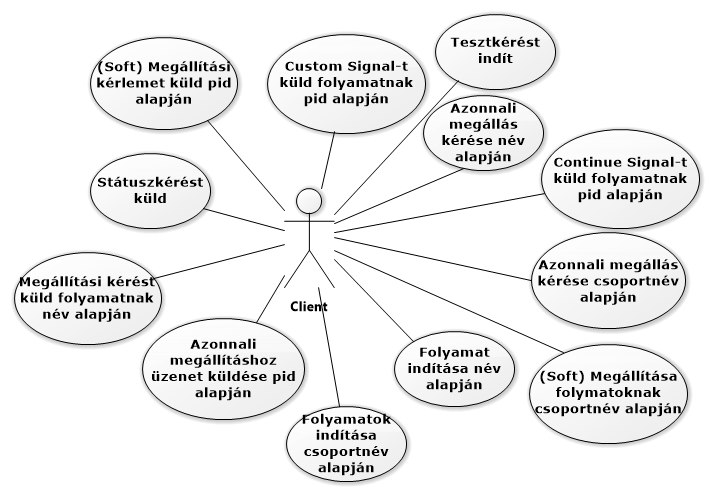
\includegraphics[width=15cm]{pics/func_uc.png}
	  \caption{A teljes kommunikációs interfész funkcionalitását bemutató ábra. \newline}
  \end{figure}
  
\subsection{Client}
\paragraph{}
A kliens komponens legfőbb feladata, hogy a feladat által megfogalmazott kommunikációs interfészt biztosítsa a felhasználójának. Ebbe beletartozik a kapcsolat megvalósítása socketen keresztül, továbbá az is, hogy felhasználói felületet biztosítson a program kezeléséhez.
    
\subsubsection{Osztályok}
A kliens az alábbi osztályokból épül fel:
\paragraph{ClientApplication} 
A ServerApplication osztály mintájárára, a kliens komponensben ez az osztály képezi az alkalmazásréteget. A feladata, hogy az érékelt parancssori paraméterek megadása után, a konfigurációs állományt feldolgozva olyan állapotba juttassa az alkalmazást, hogy az a működés magját alkotó ciklus számára alkalmas legyen. A főciklus feladata, hogy minden egyes kívánt iteráció esetén egy parancsot hajtson végre. Ezen parancsok az iteráció elején képernyőre írt menü alapján vezérelhetők. A paraméter táblázatból (\ref{tab:cli}. bekezdés) látható, hogy a \textit{help} kapcsoló megadása esetén, a program a fentebb említett ciklust mellőzve, a program paraméterezésének kiírása után leáll. Minden egyéb funkció esetén, a program a ciklusba belép, és a megfelelő navigációs utasításra vár.
Az itt megadható lehetőségek vezérlését, az ezekre kapott válaszok feldoglozását és a megfelelő I/O műveletek végrehajtását is ezen réteg adja. Lényegében a felhasználó ezen a rétegen keresztül vezérli a rendszert.
\paragraph{ClientOptions}

A kliens komponens esetében is azon alapelvek érvényesek, amelyek a szerver komponens esetében meg lettek határozva. A működés magját képező Client objektum is bizonyos opciók alapján inicializálja jellemző működését. Ezen opciókból itt lényegesen kevesebb található, mint a szerverbéli megfelelőjében. Ugyanis  a megfelelő csatlakozási címen kívül az alkalmazás konfigurácós állományának, illetve a hitelesítéshez szükséges felhasználónév és jelszó páros meghatározására van lehetőség.
\paragraph{ClientConfiguration}
Ezen osztály a ClientOptions segítségével jön létre, célja, hogy a megadott konfigurációs fájlban található beállításokat betöltse a megfelelő Options argumentumba.
\subparagraph{Megjegzés:} 
Itt is megjegyezném, hogy a konfigurációs réteg kialakításakor figyelembe lett véve, hogy esetleg JSON-től különböző állomány betöltésére is legyen a későbbiekben lehetőség.

    \begin{figure}[ht]
       \centering
         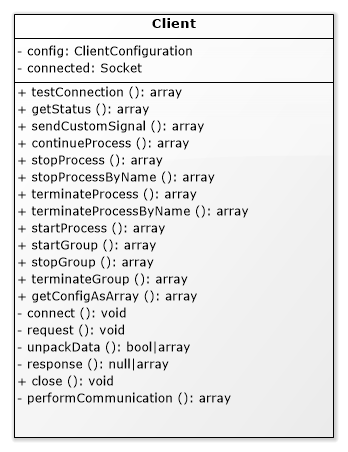
\includegraphics[width=7cm]{pics/clie.png}
	  \caption{A Client osztályt ábrázoló diagramm.}
  \end{figure}
  
\paragraph{Client}
A komponens központi működését szolgáltató objektum, aminek a feladata a kommunikációs réteg magvalósítása. Fontosabb funkciója a \verb|performCommunication|, ami egy kommunikációs kapcsolat életciklusát implementálja. Azaz kapcsolódik a kívánt címre, majd a kiválasztott menü alapján a megfelelő üzenetet küldi el, illetve fogadja a választ, és dekódolja  ClientApplication számára értelmezhető formátumra. Ezen kommunikációs ciklusok körökre osztottak, minden egyes kérés küldésre pontosan egyetlen választ vár, majd miután azt megkapta, bontja a kapcsolatot.
\subparagraph{Megjegyzés:}
Minden szerver felé közölt kérés rögzített kódú paranccsal történik, és ezáltal az átküldött üzenet mérete becsülhető felső korláttal. Ezt használja ki a Server komponens a kommunikációhoz, mert az az objektum 1024 bájtban meghatározott fogadási bufferen várja a kódolt üzenetet. Ugyanakkor, mivel a válaszüzenet mérete jóval nagyobb lehet ennél, ezért a kliens oldalon ciklusban fogadjuk a socketen érkező adatokat, ugyanúgy 1024 bájt méretű buffer segítségével.
\subparagraph{Megjegyzés:}
A kommunikáció köztes pontján, amikor a szerver dolgozik, a kliens legfeljebb 60 másodpercig vár arra, hogy a megfelelő socket olvasásra felszabaduljon.

\subsubsection{Felhasználói esetek}
   \begin{figure}[ht]
       \centering
         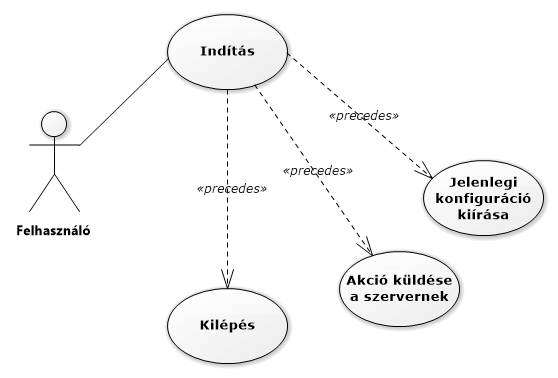
\includegraphics[width=11cm]{pics/cluc.png}
	  \caption{A kliensprogram használati esetei.}
  \end{figure}
  

\section{Megvalósítás}
A rendszer implementációja során a magasszintű konfigurálhatóság, illetve az objektum-elvű szemléletek voltak előtérbe helyezve. A megvalósított konzolos alkalmazások indító szkriptjei a megfelelő, már bemutatott objektumot példányosítva, majd azt elindítva működnek. A névterek kialakítása a PSR-4-es szabvány szerint történt, és az ezeket feloldó \textit{AutoLoader} objektum a statikus metódusai segítségével regisztrálja a megfelelően hivatkozott névtereket. Az osztály implementációja az \textit{src} mappa gyökerében található.
\subparagraph{Megjegyzés:} A manapság szokásos standardok szerint, dependency-manager-re bízott telepítés integrálásával a rendszerből kiemelhetővé (dependency-vé) válik az External könyvtár alatt található forrás-projekt. Ez egy későbbi fejlesztési időszak tárgyát képezheti. (Pl.: Composer alá)
\paragraph{Kommunikáció}
A kommunikációt a kliens komponens kezdeményezi. Jelenleg a datagram és a stream alapú socketek kommunikációja lehetséges a rendszerben. Ezen socketek a kapcsolat létrejötte után kérdés-válasz jellegű adatcserét végeznek. A szerveroldali socketek legfeljebb 1024 bájt méretű adatban fogadják az üzeneteket. A kliens oldali socket időkorlátos megvalósítással rendelkezik, ami azt jelenti, hogy amennyiben a megadott időn belül (60 másodperc) nem olvasható a válasz a socketen, bontja a kapcsolatot.
A kommunikáció során az egyes felek leellenőrzik a teljes üzenet átérkezését, s amennyiben ez teljesül, sikeresnek tekinthető az üzenetfogadás.
\subparagraph{Üzenetek}
Az üzenetek alapvetően string formába csomagolt adatok. Ezen string egy mindkét komponensben definiált tokennel kezdődik illetve végződik. A token (tag) közrezárja az egy üzenetben lévő \verb|json_encode| által szöveggé alakított tömböt. A tömb reprezentálja az üzenetet, aminek tartalma a végrehatjani kívánt akció neve, annak paramétere (ha van), továbbá a konfigurációban meghatározott felhasználónév és jelszó.
(A kiolvasási buffer mérete, ami miatt a megfelelő szöveges paraméterek (name, groupname), a felhasználónév és a jelszó is karakterlimittel van validálva.)
Az üzenetek fogadó felén, az említett token erősíti meg az üzenet megérkezését, majd a token-t eltávolítva az üzenet elejéről és végéről, a tényleges adat is kinyerhető. (Az adat \verb|json_decode| segítségével kerül elemezhető formába.) \\ \\


Egy lehetséges üzenetre példa: \\ \footnotesize
\verb|<PHPVisor>{"action":"test", "params":[], "username": null, "password": null}</PHPVisor>|
\normalsize
\subsection{Server}
A szerver komponens megvalósítása közben felmerül egy-két olyan fontosabb probléma, amelyekről érdemes említést tenni.
   \paragraph{Az öröklődési probléma}
   Az alábbi jelenség amiről szó van, a folyamatok új számítási szálra való lehelyezése miatt fordulhat elő. A probléma az, hogy a \verb|proc_open| függvény a \textit{fork} alkalmazásával helyezi le az új szálra a megadott futtatandó parancsot. A fork működése miatt \textsuperscript{\cite{fork}} a gyermekfolyamatok megöröklik a szülőfolyamat fájlleíróit. Ez azt jelenti, hogyha valamilyen oknál fogva a program futásakor a szülőfolyamatot lelövi az operációs rendszer, de egy gyermekfolyamat még várakozik (és fut), akkor az a folyamat megörökli a nyitott socketekhez tartozó leírókat is. Ezáltal a socketet még nyitottnak látszódnak, pedig tulajdonképpen nincs mögöttük a működést biztosító szál.
   
   Mivel a PHP jelenleg nem nyújt lehetőséget a megfelelő közbenjárásra a problémával kapcsolatban, ezért csak \textit{workaround} eszközölhető. Ezen eset miatt, a szerver indulásakor elinduló folyamatokat előbb indítjuk mint a socketeket, de ez nem valódi megoldás a problémára. A megoldáshoz az FD\_CLOEXEC descriptor flag alkalmazására lenne szükség, amellyel elérhető, hogy a megfelelő leíró bezárásra kerüljön és ne történjen meg az öröklődés.
   \subparagraph{Megjegyzés:}
   Amennyiben a PHP lehetőséget tud nyújtani a fent említett problémára a programot, érdemes továbbfejleszteni a megjelölt hibalehetőség kizárásával.
    
   \paragraph{Folyamatok kezelése}
   A folyamatok alapvető kezelését PHP-s függvényekkel oldottam meg. A folyamatok létrehozását a \verb|proc_open| függvény végzi. A \verb|proc_close| és a \verb|proc_terminate| függvények segítségével a normális (soft), illetve az azonnali (hard) leállítás funkciók is implementálásra kerültek. A kiválasztott futtatandó parancsot megfelelő \verb|escapeshellcmd| függvényen átvezetve passzoljuk a \verb|proc_open| számára.
   A folyamatok indításuk után folyamatosan vizsgálódnak a \verb|proc_get_status| függvény segítségével. Bizonyos értékekre a függvény nem aktuális adatokat szolgáltat, így ezt szem előtt tartva lett megvalósítva a Process objektum updateStatus, státusz frissítést végző metódusa. Ezen státusz változása esetén a megfelelő állapotot kifejező argumentum is változtatásra kerül az adott Process objektumban, hogy az megfeleltethető legyen a folyamat aktuális állapotával.
   \paragraph{A demonizáció}
   A demonizáció algoritmusa a szakirodalmakban\textsuperscript{\cite{stevens}} megtalálható lépéseket követi. A demonizáció lényege, hogy a háttérbe szorítani kívánt futási szálat leválasztjuk az aktuális terminálról, ezzel háttérbe helyezve.
   \\
   A lépések a következők\textsuperscript{\cite{daemon}}:
   \begin{enumerate}\centering\small
   		\item Fájlleírók bezárása.
        \item Vezérlő terminálról való leválasztása.
        \item Munkamenet és folyamatcsoportok elvesztése.
        \item Aktuális munkakönyvtár megváltoztatása.
        \item Újraállítani a fájlok létrehozási maszkját.
        \item Gyermekkel kapcsolatos szignál kezelése. (SIGCHLD)
   \end{enumerate}
 
 Ezen általános leírás nem minden lépésére van szükség a tényleges implementációban. A fájlleírók és a terminálról való leválasztás után (\verb|posix_setsid| függvény) a Server alkalmazás a megadott könyvtárba navigál, majd elkészíti a program pid fájlját, amibe a demonizált folyamat pid-át írja bele. Végül alkalmazza a megadott umaszk értéket, amennyiben erre van jogosultsága a futtató felhasználónak.
 \subparagraph{Megjegyzés:}
 W. Stevens az Advanced Unix könyvében SVR4 okokra hivatkozva a SIGHUP figyelmen kívül hagyását és újra-forkolást javasol a setsid hívást követően (13.3 fejezetben), de ezen működés nem része az implementációnak.\textsuperscript{\cite{stevens}}
\subsection{Client}
A kliens lényegében egy komolyabb mechanizmust valósít meg, ami a kommunikáció. Önmagában a program célja, hogy egy kezelhető felületet valósítson meg felhasználója számára, amivel vezérelni tudja a szerver komponenst.
  \paragraph{Kommunikáció}
  A kommunikációs réteg megvalósításáról már több szó is esett. A program rögzített karakterszámú üzeneteket továbbít, illetve időkorláttal vár az érkező válaszra, aminek eredményéről és sikerességéről a felhasználó számára kiírt üzenetekben tájékoztat.
  Az egyetlen érdekesnek mondható metódus az adatok fogadása, mivel nem tudhatjuk mekkora választ kell fogadnunk. Ezt egy ciklusos olvasással oldjuk meg a PHP-s \verb|socket_recv| függvény felhasználásával, amely megkülönbözteti az aktuálisan nem kapott értékek esetét, az üzenet végét jelentő esetektől. (Egy beolvasási "kör" (iteráció) bufferének mérete itt is 1024 bájt.)

\chapter{Tesztelés}
\paragraph{}
A programok tesztelését kézzel végeztem, de megtalálható több speciális konfigurációs állomány a \textit{test} könyvtár alatt, amelyek segítségvél ellenőrizhető a program egy-egy opció alkamazása esetén. A rendszer megfelelő működéséről funkciói segítségével tájékozódhatunk. A szerver esetén a képernyőre vagy naplóba írt bejegyzések segítik a futás nyomon követését, míg a kliensnél a képernyőre írt információk teszik egyértelművé a futás állapotait. 
\subparagraph{Megjegyzés:}
Egy PHP-s tesztelést segítő keretrendszer integrálásával, későbbi fejlesztések alkalmával sor kerülhet egységtesztek bevezetésére. A PHPUnit\textsuperscript{\cite{phpunit}} egy szabadon használható szoftver, amely támogatja objektumok egységteszteinek írását \textit{assert}-ek segítégével.\footnote{Az egyes tesztesetek a \textit{test} könyvtárban találhatóak}
\section{Server}
\subsection{Feketedoboz tesztesetek}
\begin{itemize}
\item Nem JSON konfigurációs fájl (nonjson.test)
\item Nem megfelelő környezetben való futtatás
\item Üres fájl (empty.test)
\item Üres JSON fájl (empty.test.json)
\item Invalid érték a logikai értékek helyett (invalidValues.test.json)
\item Invalid érték a szám értékek helyett (invalidValues.test.json)
\end{itemize}
\subsection{Fehérdoboz tesztesetek}
\begin{itemize}
\item Minimális kötelező konfigurációval való működés (requireds.test.json)
\item Hiányzó socket konfiguráció (misssock.test.json)
\item Hiányzó process konfiguráció (missproc.test.json)
\item Hiba esetén a naplóba íródik a megfelelő hibaüzenet. (misssock.test.json)
\item Túl hosszú limitált érték (pl. name) (tooLongName.test.json)
\item Megfelelő újraindítási szabályok lépnek életbe adott folyamat egy lefutásakor (run.test.json)
\end{itemize}
\section{Client}
\subsection{Feketedoboz tesztesetek}
\begin{itemize}
\item Hibás parancssori konfiguráció beütése
\item Nem JSON konfigurációs fájl (nonjson.test)
\item Üres fájl (empty.test)
\item Üres JSON fájl (empty.test.json)
\item Túl hosszú felhasználónév megadása fájlban (tooLongUsername.test.json)
\item Túl hosszú akcióparaméterek tesztje
\item Hibás menüopció választása
\end{itemize}
\subsection{Fehérdoboz tesztesetek}
Mivel a kliensnek meglehetősen kevés konfiguációs beállítása van, ezért az itt ugyanúgy érvényes teszteseteket nem sorolom fel. A kliens funkcionális tesztelése keretében a letesztelt funkciók:
\begin{itemize}
\item Test menü működése
\item Custom menü működése
\item Folyamatok indítása pid/név/csoportnév alapján
\item Folyamatok leállítása pid/név/csoportnév alapján
\item Folyamatok terminálása pid/név/csoportnév alapján
\item Folyamat folytatása Stopped állapot esetén
\item Állapot lekérdezése
\item Kapcsolat megszakadása esetén érkező hibák
\end{itemize}

\section{Hatékonyság}
A program hatékonyságát több szempont alapján elemezhetjük. A kommunikációs részprogram erőforráskímélő, mivel a randevú a lehető legrövidebb ideig tart. Ugyanakkor a hálózat paraméteritől is függ, hogy milyen sebességgel képes továbbítani az adatokat az adott komponens.
A folyamatkezelő mechanizmus a futó folyamatokat pid-re kulcsolt tömbben tárolja, így azok elérése egy-egy interakció esetén a lehető leggyorsabb. Ugyanakkor az összes folyamatot tároló tömb nem kulcsolt, így név vagy csoportnév alapján folyamatok meghatározása keresést igényel.
A rendszer megvalósítása során, a már nem használt objektumok/referenciák felszabadításra kerülnek, ezáltal a PHP nyújtotta Garbage Collector szolgáltatásra bízva a takarítást.
  
\chapter{Zárszó} 
\paragraph{}
A PHPVisor megszületését az ösztönözte, hogy komplexebb összetételű alkalmazások működése során külső, illetve független programkomponensek lefutására lehet szükség.
Az egyes futtatandó programok ideális esetben ritkán változnak, ezzel ellentétben a lefutásukra jelentkező igény különféle üzleti helyzetekben, különféle ütemezést jelenthet.
Ilyen esetekben egy megfelelő folyamatkezelést, vezérlést biztosító program megléte rendkívül megkönnyítheti az üzemeltetést. A program implementációjából fakadóan minimális függőséget jelenthet alkalmazási környezettől függően.
\paragraph{}
A tervezett céljaim a program megvalósítása során teljesültek. Az eleinte kitalált funkcionalitások implementálásra kerültek, továbbá olyan funkciók is megvalósultak, amelyek a kényelmesebb használatot teszik lehetővé.
Az alapvető irányvonal a fejlesztés során az volt, hogy egy egyszerűen kezelhető programot hozzak létre, ami magasszintű konfigurálhatóságot biztosít a felhasználójának.
A fejlesztés jelenlegi iránya, hogy még több olyan funkció kerüljön a rendszerbe, amelyek elősegítik a gördülékeny használatot. 

A jövőre mutató tervek között szerepel egy automatikus verziózó szolgáltatás implementálása a szerver komponens számára, de egy alternatív kliens is, ami egy grafikus felületű kezelő-(web)oldalt szolgáltat a rendszer vezérléséhez.
További fejlesztési munkálatok során ki lehetne terjeszteni a szerver kommunikációs lehetőségeit más specifikusabb protkollokra, HTTP-n keresztüli üzenetváltási standardeket implementálni, esetleg egy összetettebb folyamatcsoportokat kezelő logikát integrálni.


\begin{thebibliography}{20}

\bibitem{supervisor}
  Supervisor honlapja és GitHub oldala: \\
   \hspace*{3mm}http://supervisord.org/  (2018. április 29.)\\
  \hspace*{3mm}https://github.com/Supervisor/supervisor (2018. április 29.)

\bibitem{phpcli}
  PHP CLI honlapja: \\
   \hspace*{3mm}http://php.net/manual/en/features.commandline.php  (2018. május 03.)
   
\bibitem{phppcntl}
   PHP PCNTL: \\
   \hspace*{3mm}http://php.net/manual/en/book.pcntl.php  (2018. május 03.)
   
\bibitem{phppos}
   PHP POSIX: \\
   \hspace*{3mm}http://php.net/manual/en/book.posix.php  (2018. május 03.)
   
\bibitem{phpsock}
   PHP Socket: \\
   \hspace*{3mm}http://php.net/manual/en/book.sockets.php  (2018. május 03.)
   
\bibitem{cluesocket}
	Clue GitHub oldalán a php-socker-raw library: \\
	\hspace*{3mm}https://github.com/clue/php-socket-raw  (2018. május 05.)
    
\bibitem{fork}
	Fork manual oldala: \\
	\hspace*{3mm} https://linux.die.net/man/2/fork  (2018. május 05.)
    
\bibitem{daemon}
	Demonizálási lépések leírása az UWE oldalán: \\
	\hspace*{3mm} http://www.cems.uwe.ac.uk/\~irjohnso/coursenotes/lrc/system/daemons/d3.htm  (2018. május 06.)
    
\bibitem{stevens}
	W. R. Stevens: Advanced programming in the UNIX environment \\
    - Third Edition -, Addison Wesley, 2013, [994], ISBN-13: 978-0-321-63773-4 
    
\bibitem{phpunit}
	PHPUnit tesztelési keretrendszer oldala: \\
	\hspace*{3mm}https://phpunit.de/  (2018. május 09.)
    
\end{thebibliography}

\end{document}